%\documentclass[12pt]{article}

\newcommand{\he}{\hat{\mathbf{e}}}

\questionheader{ex:s3.2}


%%%%%%%%%%%%%%%%%%
\subsection*{\Conceptual}
%%%%%%%%%%%%%%%%%%

%%%%%%%%%%%%%%%%%%%%%%%%%%%%
%\Instructions{Questions~\ref{prob_s1.0first} through \ref{prob_s1.0last} provide practice with.}
%%%%%%%%%%%%%%%%%%%%

%%%%%%%%%%%%%%%%%%%%%%%%%%%
\begin{question}
Consider the points
\begin{align*}
(x_1,y_1) &= (3,0) &
(x_2,y_2) &= (1,1)  &
(x_3,y_3) &= (0,1) \\
(x_4,y_4) &= (-1,1) &
(x_5,y_5) &= (-2,0)
\end{align*}
For each $1\le i\le 5$, 
\begin{itemize}
\item
sketch, in the $xy$-plane, the point $(x_i,y_i)$ and
\item
find polar coordinates $r_i$ and $\theta_i$,
with $r_i>0$ and $0\le\theta_i<2\pi$, for the point $(x_i,y_i)$.
\end{itemize}
\end{question}

%\begin{hint} 
%\end{hint}

\begin{answer} 
The left hand sketch below contains the points, $(x_1,y_1)$, $(x_3,y_3)$,
$(x_5,y_5)$, that are on the axes. The right hand sketch below contains the
points, $(x_2,y_2)$, $(x_4,y_4)$, that are not on the axes.
\begin{center}
  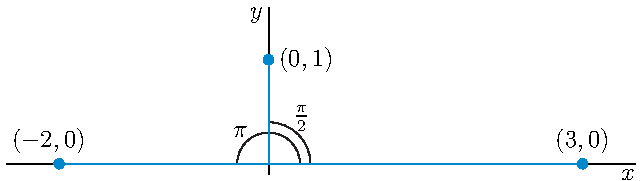
\includegraphics[scale=0.95]{polar3A.pdf}\quad
  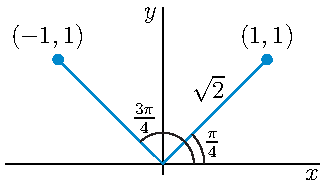
\includegraphics[scale=0.95]{polar2A.pdf}
\end{center}
    $r_1 = 3$,        $\theta_1=0$\qquad 
    $r_2 = \sqrt{2}$, $\theta_2=\frac{\pi}{4}$\qquad 
    $r_3 = 1$,        $\theta_3=\frac{\pi}{2}$\qquad 
    $r_4 = \sqrt{2}$, $\theta_4=\frac{3\pi}{4}$\\
    $r_5 = 2$,        $\theta_5=\pi$
\end{answer}


\begin{solution}
The left hand sketch below contains the points, $(x_1,y_1)$, $(x_3,y_3)$,
$(x_5,y_5)$, that are on the axes. The right hand sketch below contains the
points, $(x_2,y_2)$, $(x_4,y_4)$, that are not on the axes.
\begin{center}
  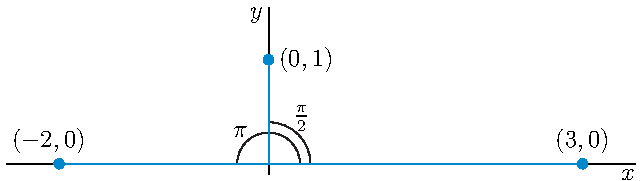
\includegraphics[scale=0.95]{polar3A.pdf}\quad
  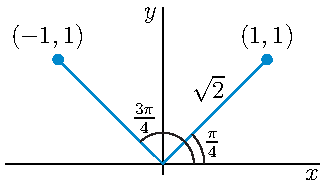
\includegraphics[scale=0.95]{polar2A.pdf}
\end{center}
Recall that the polar coordinates $r$, $\theta$
are related to the cartesian coordinates $x$, $y$, by $x=r\cos\theta$,
$y=r\sin\theta$. So $r=\sqrt{x^2+y^2}$ and $\tan\theta=\frac{y}{x}$
(assuming that $x\ne 0$ and $r>0$) and
\begin{alignat*}{5}
(x_1,y_1) &= (3,0) &&\implies &r_1=3,\ \tan\theta_1=0
                   &&\implies \theta_1&=0 
                   \text{ as $(x_1,y_1)$ is on the positive $x$-axis} \\
(x_2,y_2) &= (1,1) &&\implies &r_2=\sqrt{2},\ \tan\theta_2=1
                   &&\implies \theta_2&=\frac{\pi}{4} 
                   \text{ as $(x_2,y_2)$ is in the first octant} \\
(x_3,y_3) &= (0,1) &&\implies &r_3=1,\ \cos\theta_3=0
                   &&\implies \theta_3&=\frac{\pi}{2} 
                   \text{ as $(x_3,y_3)$ is on the positive $y$-axis} \\
(x_4,y_4) &= (-1,1) &&\implies &r_4=\sqrt{2},\ \tan\theta_4=-1
                   &&\implies \theta_4&=\frac{3\pi}{4} 
                   \text{ as $(x_4,y_4)$ is in the third octant} \\
(x_5,y_5) &= (-2,0) &&\implies &r_5=2,\ \tan\theta_5=0
                   &&\implies \theta_5&=\pi 
                   \text{ as $(x_5,y_5)$ is on the negative $x$-axis} 
\end{alignat*}
\end{solution}


%%%%%%%%%%%%%%%%%%%%%%%%%%%
\begin{question}
For each of the following points $(x_i,y_i)$,
\begin{itemize}
\item
find \emph{all} pairs $(r_i,\theta_i)$ such that 
  $(x_i,y_i) = \big(r_i\cos\theta_i\,,\,r_i\sin\theta_i\big)$, and
\item
 in particular, find a pair $(r_i,\theta_i)$ with $r_i<0$ and 
$0\le\theta_i<2\pi$ such that 
  $(x_i,y_i) = \big(r_i\cos\theta_i\,,\,r_i\sin\theta_i\big)$
\end{itemize}

\begin{enumerate}[(a)]
\item
$ (x_1,y_1) = (-2,0) $ 
\item
$ (x_2,y_2) = (1,1) $ 
\item
$ (x_3,y_3) = (-1,-1) $ 
\item
$ (x_4,y_4) = (3,0) $ 
\item
$ (x_5,y_5) = (0,1) $ 
\end{enumerate}
\end{question}

\begin{hint} 
$r$ is allowed to be negative.
\end{hint}

\begin{answer} 
(a) $\big(r_1=2\,,\,\theta_1= n\pi,\ n\text{ odd integer }\big)$ or 
    $\big(r_1=-2\,,\,\theta_1= n\pi,\ n\text{ even integer }\big)$.
    In particular,  $\big(r_1=-2\,,\,\theta_1= 0\big)$ has $r_1<0$
    and $0\le\theta_1<2\pi$.

(b) $\big(r_2=\sqrt{2}\,,\,\theta_2= \nicefrac{\pi}{4} + 2n\pi\big)$ or 
    $\big(r_2=-\sqrt{2}\,,\,\theta_2= \nicefrac{5\pi}{4} + 2n\pi\big)$,
    with $n$ integer. In particular,  $\big(r_2=-\sqrt{2}\,,\,
    \theta_2= \nicefrac{5\pi}{4}\big)$ has $r_2<0$
    and $0\le\theta_2<2\pi$.

(c) $\big(r_3=\sqrt{2}\,,\,\theta_3= \nicefrac{5\pi}{4} + 2n\pi\big)$ or 
    $\big(r_3=-\sqrt{2}\,,\,\theta_3= \nicefrac{\pi}{4} + 2n\pi\big)$,
    with $n$ integer. In particular,  $\big(r_3=-\sqrt{2}\,,\,
    \theta_3= \nicefrac{\pi}{4}\big)$ has $r_3<0$
    and $0\le\theta_3<2\pi$.

(d) $\big(r_4=3\,,\,\theta_4= 0 + 2n\pi\big)$ or 
    $\big(r_4=-3\,,\,\theta_4= \pi + 2n\pi\big)$,
    with $n$ integer. In particular,  $\big(r_4=-3\,,\,
    \theta_4= \pi\big)$ has $r_4<0$ and $0\le\theta_4<2\pi$.

(e) $\big(r_5=1\,,\,\theta_5= \nicefrac{\pi}{2} + 2n\pi\big)$ or 
    $\big(r_5=-1\,,\,\theta_5= \nicefrac{3\pi}{2} + 2n\pi\big)$,
    with $n$ integer. In particular,  $\big(r_5=-1\,,\,
    \theta_5= \nicefrac{3\pi}{2}\big)$ has $r_5<0$
    and $0\le\theta_5<2\pi$.
\end{answer}


\begin{solution}
In this solution, we'll supress the subscripts. That is, we'll write $r$ in place of $r_i$ and $\theta$ in place of $\theta_i$.
Note that the distance from the point $\big(r\cos\theta\,,\,r\sin\theta\big)$
to the origin is
\begin{equation*}
\sqrt{r^2\cos^2\theta + r^2\sin^2\theta}
=\sqrt{r^2}
=|r|
\end{equation*}
Thus $r$ can be either the distance to the origin or minus the distance to the
origin.

(a) 
The distance from $(-2,0)$ to the origin is $2$. So either $r=2$ or $r=-2$.
\begin{itemize}
\item If $r=2$, then $\theta$ must obey 
\begin{align*}
(-2,0) = \big(2\cos\theta\,,\,2\sin\theta\big)
&\iff \sin\theta=0,\ \cos\theta=-1 \\
&\iff \theta= n\pi,\ n\text{ integer },\ \cos\theta=-1 \\
&\iff \theta= n\pi,\ n\text{ odd integer }
\end{align*}
\item If $r=-2$, then $\theta$ must obey 
\begin{align*}
(-2,0) = \big(-2\cos\theta\,,\,-2\sin\theta\big)
&\iff \sin\theta=0,\ \cos\theta=1 \\
&\iff \theta= n\pi,\ n\text{ integer },\ \cos\theta=1 \\
&\iff \theta= n\pi,\ n\text{ even integer }
\end{align*}
\end{itemize}
In particular,  $\big(r=-2\,,\,\theta= 0\big)$ has $r<0$
    and $0\le\theta<2\pi$.

In the figure on the left below, the blue half-line is the set of all points 
with polar coordinates $\theta=\pi$, $r>0$ and the orange half-line is the set 
of all points  with polar coordinates $\theta=\pi$, $r<0$. 
In the figure on the right below, the blue half-line is the set of all points 
with polar coordinates $\theta=0$, $r>0$ and the orange half-line is the set 
of all points  with polar coordinates $\theta=0$, $r<0$. 
\begin{center}
  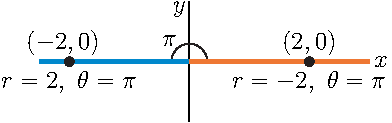
\includegraphics{polar6BB.pdf}\qquad
  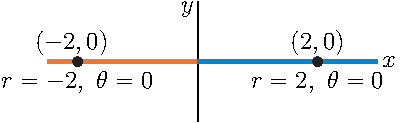
\includegraphics{polar6AA.pdf}
\end{center}


(b)
The distance from $(1,1)$ to the origin is $\sqrt{2}$. 
So either $r=\sqrt{2}$ or $r=-\sqrt{2}$.
\begin{itemize}
\item If $r=\sqrt{2}$, then $\theta$ must obey 
\begin{align*}
(1,1) = \big(\sqrt{2}\,\cos\theta\,,\,\sqrt{2}\,\sin\theta\big)
&\iff \sin\theta=\cos\theta=\nicefrac{1}{\sqrt{2}} \\
&\iff \theta= \nicefrac{\pi}{4} + 2n\pi,\ n\text{ integer }
\end{align*}
\item If $r=-\sqrt{2}$, then $\theta$ must obey 
\begin{align*}
(1,1) = \big(-\sqrt{2}\,\cos\theta\,,\,-\sqrt{2}\,\sin\theta\big)
&\iff \sin\theta=\cos\theta=-\nicefrac{1}{\sqrt{2}} \\
&\iff \theta= \nicefrac{5\pi}{4} + 2n\pi,\ n\text{ integer }
\end{align*}
\end{itemize}
In particular,  $\big(r=-\sqrt{2}\,,\,
    \theta= \nicefrac{5\pi}{4}\big)$ has $r<0$
    and $0\le\theta<2\pi$.

In the figure on the left below, the blue half-line is the set of all points 
with polar coordinates $\theta=\frac{\pi}{4}$, $r>0$ and the orange half-line 
is the set of all points  with polar coordinates $\theta=\frac{\pi}{4}$, $r<0$. 
In the figure on the right below, the blue half-line is the set of all points 
with polar coordinates $\theta=\frac{5\pi}{4}$, $r>0$ and the orange 
half-line is the set of all points  with polar coordinates 
$\theta=\frac{5\pi}{4}$, $r<0$. 
\begin{center}
  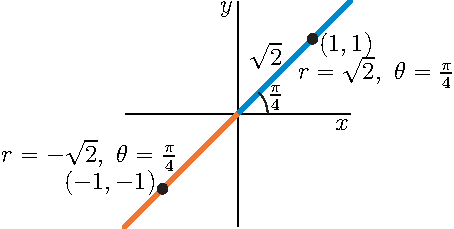
\includegraphics{polar4AA.pdf}\qquad
  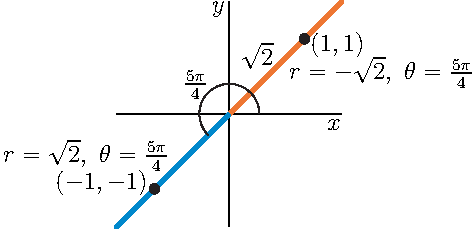
\includegraphics{polar4BB.pdf}
\end{center}

(c)
The distance from $(-1,-1)$ to the origin is $\sqrt{2}$. 
So either $r=\sqrt{2}$ or $r=-\sqrt{2}$.
\begin{itemize}
\item If $r=\sqrt{2}$, then $\theta$ must obey 
\begin{align*}
(-1,-1) = \big(\sqrt{2}\,\cos\theta\,,\,\sqrt{2}\,\sin\theta\big)
&\iff \sin\theta=\cos\theta=-\nicefrac{1}{\sqrt{2}} \\
&\iff \theta= \nicefrac{5\pi}{4} + 2n\pi,\ n\text{ integer }
\end{align*}
\item If $r=-\sqrt{2}$, then $\theta$ must obey 
\begin{align*}
(-1,-1) = \big(-\sqrt{2}\,\cos\theta\,,\,-\sqrt{2}\,\sin\theta\big)
&\iff \sin\theta=\cos\theta=\nicefrac{1}{\sqrt{2}} \\
&\iff \theta= \nicefrac{\pi}{4} + 2n\pi,\ n\text{ integer }
\end{align*}
\end{itemize}
In particular,  $\big(r=-\sqrt{2}\,,\,
    \theta= \nicefrac{\pi}{4}\big)$ has $r<0$
    and $0\le\theta<2\pi$.

In the figure on the left below, the blue half-line is the set of all points 
with polar coordinates $\theta=\frac{5\pi}{4}$, $r>0$ and the orange half-line 
is the set of all points  with polar coordinates 
$\theta=\frac{5\pi}{4}$, $r<0$. 
In the figure on the right below, the blue half-line is the set of all points 
with polar coordinates $\theta=\frac{\pi}{4}$, $r>0$ and the orange 
half-line is the set of all points  with polar coordinates 
$\theta=\frac{\pi}{4}$, $r<0$. 
\begin{center}
  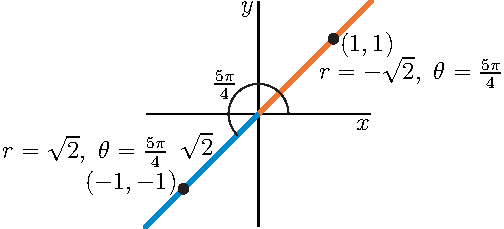
\includegraphics[scale=0.9]{polar5AA.pdf}\qquad
  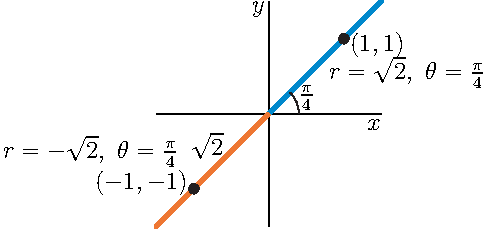
\includegraphics[scale=0.9]{polar5BB.pdf}
\end{center}

(d)
The distance from $(3,0)$ to the origin is $3$. 
So either $r=3$ or $r=-3$.
\begin{itemize}
\item If $r=3$, then $\theta$ must obey 
\begin{align*}
(3,0) = \big(3\,\cos\theta\,,\,3\,\sin\theta\big)
&\iff \sin\theta=0,\ \cos\theta=1 \\
&\iff \theta= 0 + 2n\pi,\ n\text{ integer }
\end{align*}
\item If $r=-3$, then $\theta$ must obey 
\begin{align*}
(3,0) = \big(-3\,\cos\theta\,,\,-3\,\sin\theta\big)
&\iff \sin\theta=0,\ \cos\theta=-1 \\
&\iff \theta= \pi + 2n\pi,\ n\text{ integer }
\end{align*}
\end{itemize}
In particular,  $\big(r=-3\,,\,
    \theta= \pi\big)$ has $r<0$
    and $0\le\theta<2\pi$.

In the figure on the left below, the blue half-line is the set of all points 
with polar coordinates $\theta=\pi$, $r>0$ and the orange half-line is the set 
of all points  with polar coordinates $\theta=\pi$, $r<0$. 
In the figure on the right below, the blue half-line is the set of all points 
with polar coordinates $\theta=0$, $r>0$ and the orange half-line is the set 
of all points  with polar coordinates $\theta=0$, $r<0$. 
\begin{center}
  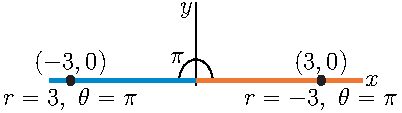
\includegraphics{polar3AA.pdf}\qquad
  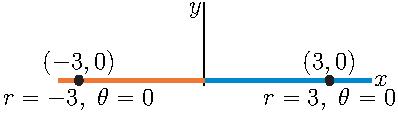
\includegraphics{polar3BB.pdf}
\end{center}

(e)
The distance from $(0,1)$ to the origin is $1$. 
So either $r=1$ or $r=-1$.
\begin{itemize}
\item If $r=1$, then $\theta$ must obey 
\begin{align*}
(0,1) = \big(\cos\theta\,,\,\sin\theta\big)
&\iff \cos\theta=0,\ \sin\theta=1 \\
&\iff \theta= \nicefrac{\pi}{2} + 2n\pi,\ n\text{ integer }
\end{align*}
\item If $r=-1$, then $\theta$ must obey 
\begin{align*}
(0,1) = \big(-\cos\theta\,,\,-\sin\theta\big)
&\iff \cos\theta=0,\ \sin\theta=-1 \\
&\iff \theta= \nicefrac{3\pi}{2} + 2n\pi,\ n\text{ integer }
\end{align*}
\end{itemize}
In particular,  $\big(r=-1\,,\,
    \theta= \nicefrac{3\pi}{2}\big)$ has $r<0$
    and $0\le\theta<2\pi$.

In the figure on the left below, the blue half-line is the set of all points 
with polar coordinates $\theta=\frac{3\pi}{2}$, $r>0$ and the orange half-line is the set 
of all points  with polar coordinates $\theta=\frac{3\pi}{2}$, $r<0$. 
In the figure on the right below, the blue half-line is the set of all points 
with polar coordinates $\theta=\frac{\pi}{2}$, $r>0$ and the orange half-line is the set 
of all points  with polar coordinates $\theta=\frac{\pi}{2}$, $r<0$. 
\begin{center}
  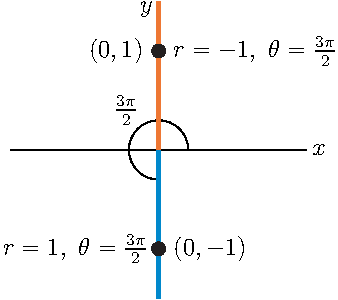
\includegraphics{polar2AA.pdf}\qquad
  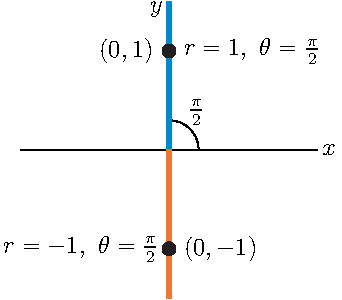
\includegraphics{polar2BB.pdf}
\end{center}


\end{solution}



%%%%%%%%%%%%%%%%%%%%%%%%%%%
\begin{question}\label{prb polar vectors}
Consider the points
\begin{align*}
(x_1,y_1) &= (3,0) &
(x_2,y_2) &= (1,1)  &
(x_3,y_3) &= (0,1) \\
(x_4,y_4) &= (-1,1) &
(x_5,y_5) &= (-2,0)
\end{align*}
Also define, for each angle $\theta$, the vectors
\begin{align*}
\he_r(\theta)=\cos\theta\ \hi + \sin\theta\ \hj\qquad
\he_\theta(\theta) = -\sin\theta\ \hi + \cos\theta\ \hj
\end{align*}
\begin{enumerate}[(a)]
\item
Determine, for each angle $\theta$, the lengths of the vectors
$\he_r(\theta)$ and $\he_\theta(\theta)$ and the angle between 
the vectors $\he_r(\theta)$ and $\he_\theta(\theta)$. Compute
$\he_r(\theta)\times\he_\theta(\theta)$ (viewing $\he_r(\theta)$ and $\he_\theta(\theta)$ as vectors in three dimensions with zero $\hk$ 
components).
\item
For each $1\le i\le 5$, sketch, in the $xy$-plane, the point 
$(x_i,y_i)= \big(r_i\cos\theta_i\,,\,r_i\sin\theta_i\big)$
and the vectors $\he_r(\theta_i)$ and $\he_\theta(\theta_i)$. In your
sketch of the vectors, place the tails of the vectors 
$\he_r(\theta_i)$ and $\he_\theta(\theta_i)$ at $(x_i,y_i)$.
\end{enumerate}
\end{question}

\begin{hint} 
Compute, for each angle $\theta$, the dot product $\he_r(\theta)\cdot\he_\theta(\theta)$.
\end{hint}

\begin{answer} 
(a) Both $\he_r(\theta)$ and $\he_\theta(\theta)$ have length 1.
The angle between them is $\frac{\pi}{2}$. The cross product is
$\he_r(\theta) \times \he_\theta(\theta)=\hk$.

(b)
Here is a sketch of $(x_i,y_i)$, $\he_r(\theta_i)$,
$\he_\theta(\theta_i)$ for $i =1,3,5$ (the points on the axes)
\begin{center}
  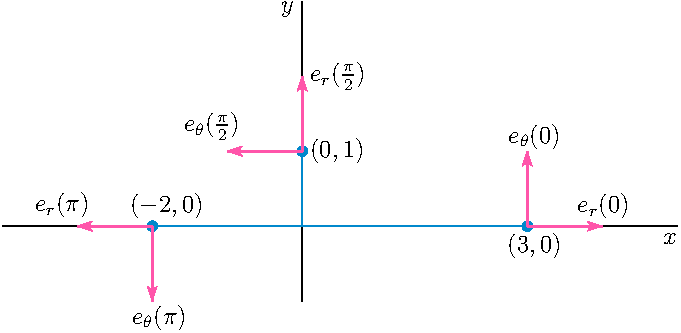
\includegraphics{polar3.pdf}
\end{center}
and here is a sketch (to a different scale) of $(x_i,y_i)$, $\he_r(\theta_i)$,
$\he_\theta(\theta_i)$ for $i =2,4$ (the points off the axes).
\begin{center}       
  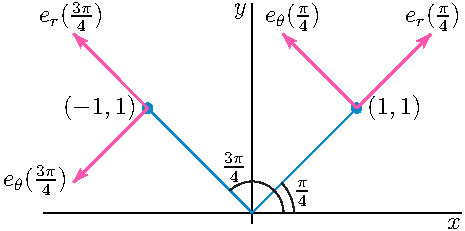
\includegraphics{polar2.pdf}
\end{center}
\end{answer}


\begin{solution} 
(a) The lengths are
\begin{align*}
|\he_r(\theta)| &= \sqrt{\cos^2\theta+\sin^2\theta} = 1 \\
|\he_\theta(\theta)| &= \sqrt{(-\sin\theta)^2+\cos^2\theta} = 1 
\end{align*}
As 
\begin{equation*}
\he_r(\theta) \cdot \he_\theta(\theta) = (\cos\theta)(-\sin\theta)
                                        +(\sin\theta)(\cos\theta)=0
\end{equation*}
the two vectors are perpendicular and the angle between them is 
$\frac{\pi}{2}$. The cross product is
\begin{align*}
\he_r(\theta) \times \he_\theta(\theta)
&=\det\left[\begin{matrix}
                  \hi  &  \hj        & \hk \\
           \cos\theta  & \sin\theta  &  0  \\
          -\sin\theta  & \cos\theta  &  0
            \end{matrix}\right] =\hk
\end{align*}

(b) Note that for $\theta$ determined by $x=r\cos\theta$, $y=r\sin\theta$,
\begin{itemize}\itemsep1pt \parskip0pt \parsep0pt %\itemindent-15pt
\item
the vector $\he_r(\theta)$ is a unit vector in the same direction as the
vector from $(0,0)$ to $(x,y)$ and 
\item
the vector $\he_\theta(\theta)$ is a unit vector that is perpendicular 
to $\he_r(\theta)$. 
\item
The $y$-component of $\he_\theta(\theta)$ has the same sign 
as the $x$-component of $\he_r(\theta)$.
The $x$-component of $\he_\theta(\theta)$ has opposite sign to that of the $y$-component  of $\he_r(\theta)$. 
\end{itemize}
Here is a sketch of $(x_i,y_i)$, $\he_r(\theta_i)$,
$\he_\theta(\theta_i)$ for $i =1,3,5$ (the points on the axes)
\begin{center}
  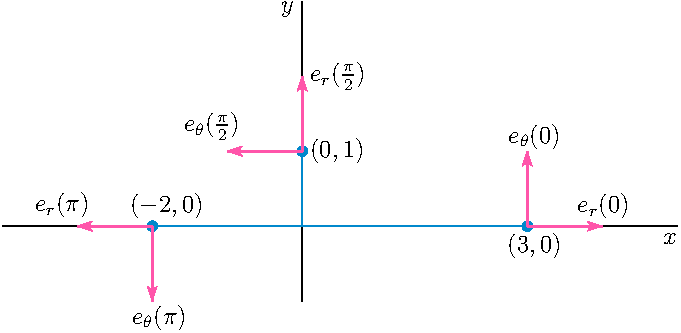
\includegraphics{polar3.pdf}
\end{center}
and here is a sketch (to a different scale) of $(x_i,y_i)$, $\he_r(\theta_i)$,
$\he_\theta(\theta_i)$ for $i =2,4$ (the points off the axes).
\begin{center}       
  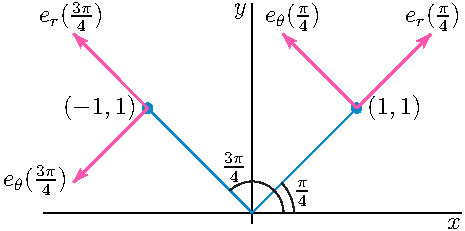
\includegraphics{polar2.pdf}
\end{center}
\end{solution}

%%%%%%%%%%%%%%%%%%%%%%%%%%%%%%%%
\begin{question}
Let $\llt a, b\rgt$ be a vector. Let $r$ be the length of $\llt a, b\rgt$
and $\theta$ be the angle between $\llt a, b\rgt$ and the $x$-axis.
\begin{enumerate}[(a)]
\item
Express $a$ and $b$ in terms of $r$ and $\theta$.
\item 
Let $\llt A, B\rgt$ be the vector gotten by rotating $\llt a, b\rgt$ 
by an angle $\varphi$ about its tail. Express $A$ and $B$ in terms of $a$, 
$b$ and $\varphi$.
\end{enumerate}
\end{question}

\begin{hint}
Sketch $\llt a, b\rgt$ and $\llt A, B\rgt$.
The trigonometric addition formulas 
\begin{align*}
\sin(\theta+\varphi)
       &=\sin\theta\cos\varphi+\cos\theta\sin\varphi \\
\cos(\theta+\varphi)
       &=\cos\theta\cos\varphi-\sin\theta\sin\varphi
\end{align*}
will help.
\end{hint}

\begin{answer}
(a) $a=r\cos\theta$, $b=r\sin\theta$

(b) $A=a\cos\varphi-b\sin\varphi$, 
    $B=b\cos\varphi+a\sin\varphi$
\end{answer}

\begin{solution}
Here is a sketch of $\llt a, b\rgt$ and $\llt A, B\rgt$.
\begin{center}
     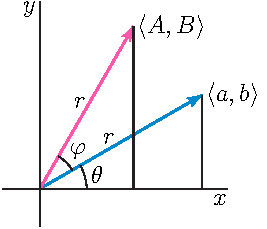
\includegraphics{polar4.pdf}
\end{center}
(a) From the sketch,
\begin{align*}
a&=r\cos\theta\\
b&=r\sin\theta
\end{align*}

(b) The length of the vector $\llt A, B\rgt$ is again $r$
and the angle between $\llt A, B\rgt$ and the $x$-axis is $\theta
+\varphi$. So
\begin{alignat*}{3}
A&=r\cos(\theta+\varphi)
&&=r\cos\theta\cos\varphi-r\sin\theta\sin\varphi
&&=a\cos\varphi-b\sin\varphi\\
B&=r\sin(\theta+\varphi)
&&=r\sin\theta\cos\varphi+r\cos\theta\sin\varphi
&&=b\cos\varphi+a\sin\varphi
\end{alignat*}

\end{solution}

%%%%%%%%%%%%%%%%%%%%%%%%%%%%%%%%%%%%%%%%%%%%%%%%%%%%%%%
\begin{question}
For each of the regions $\cR$ sketched below, express 
$\dblInt_\cR f(x,y)\,\dee{x}\,\dee{y}$ as an iterated integral in polar 
coordinates in two different ways.
\begin{center}
    (a)\quad \raisebox{-0.9\height}{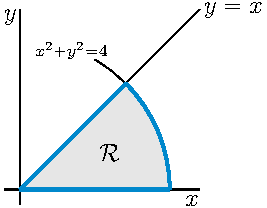
\includegraphics{polar5a1.pdf}}\hfil
    (b)\quad \raisebox{-0.9\height}{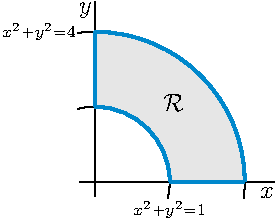
\includegraphics{polar5b1.pdf}}
\end{center}
\begin{center}
    (c)\quad \raisebox{-0.9\height}{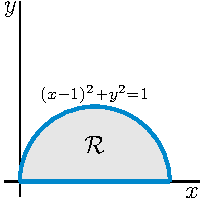
\includegraphics{polar5e1.pdf}}
                                                      \phantom{$y=x$}\hfil
    (d)\quad \raisebox{-0.9\height}{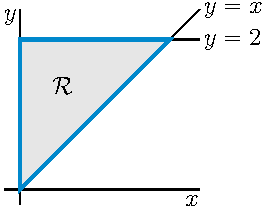
\includegraphics{polar5c1.pdf}}
\end{center}
\end{question}

%\begin{hint}
%\end{hint}

\begin{answer}

(a)
$\displaystyle\dblInt_\cR f(x,y)\,\dee{x}\,\dee{y}
=\int_0^{\nicefrac{\pi}{4}}\dee{\theta}
 \int_0^2\dee{r}\ r\ f(r\cos\theta,r\sin\theta)
=\int_0^2\dee{r}
  \int_0^{\nicefrac{\pi}{4}}\dee{\theta}
 \ r\ f(r\cos\theta,r\sin\theta)$

(b)
$\displaystyle\dblInt_\cR f(x,y)\,\dee{x}\,\dee{y}
=\int_0^{\nicefrac{\pi}{2}}\dee{\theta}
 \int_1^2\dee{r}\ r\ f(r\cos\theta,r\sin\theta)
=\int_1^2\dee{r}
  \int_0^{\nicefrac{\pi}{2}}\dee{\theta}
 \ r\ f(r\cos\theta,r\sin\theta)$

(c)
$\displaystyle \dblInt_\cR f(x,y)\,\dee{x}\,\dee{y}
=\int_0^{\nicefrac{\pi}{2}}\dee{\theta}
 \int_0^{2\cos\theta}\dee{r}\ r\ f(r\cos\theta,r\sin\theta)
=\int_0^2\dee{r}
  \int_0^{\arccos\frac{r}{2}}\dee{\theta}
 \ r\ f(r\cos\theta,r\sin\theta)$

(d)
\begin{align*}
\dblInt_\cR f(x,y)\,\dee{x}\,\dee{y}
&=\int_{\nicefrac{\pi}{4}}^{\nicefrac{\pi}{2}}\dee{\theta}
 \int_0^{\nicefrac{2}{\sin\theta}}\dee{r}\ r\ f(r\cos\theta,r\sin\theta)\\
&=\int_0^2\dee{r}
  \int_{\nicefrac{\pi}{4}}^{\nicefrac{\pi}{2}}\dee{\theta}
 \ r\ f(r\cos\theta,r\sin\theta)
+\int_2^{2\sqrt{2}}\dee{r}
  \int_{\nicefrac{\pi}{4}}^{\arcsin\frac{2}{r}}\dee{\theta}
 \ r\ f(r\cos\theta,r\sin\theta)
\end{align*}

\end{answer}

\begin{solution}
(a) The region 
\begin{equation*}
\cR=\Set{(x,y)}{0\le x^2+y^2\le 4,\ 0\le y\le x}
\end{equation*}
In polar coordinates, 
\begin{itemize}
\item
the circle $x^2+y^2=4$ becomes $r^2=4$ or $r=2$ and 
\item
the line $y=x$ becomes $r\sin\theta=r\cos\theta$ or $\tan\theta=1$ 
or $\theta=\frac{\pi}{4}$. 
\end{itemize}
Thus the domain of integration is
\begin{equation*}
\cR=\Set{(r\cos\theta,r\sin\theta)}{0\le r\le 2,\ 0\le\theta\le\tfrac{\pi}{4}}
\end{equation*}
On this domain,
\begin{itemize}
\item 
$\theta$ runs from $0$ to $\frac{\pi}{4}$. 
\item
For each fixed $\theta$ in that range, $r$ runs from $0$ to $2$, 
as in the figure on the left below.
\end{itemize}
In polar coordinates $\dee{x}\,\dee{y} = r\,\dee{r}\,\dee{\theta}$, so that
\begin{equation*}
\dblInt_\cR f(x,y)\,\dee{x}\,\dee{y}
=\int_0^{\nicefrac{\pi}{4}}\dee{\theta}
 \int_0^2\dee{r}\ r\ f(r\cos\theta,r\sin\theta)
\end{equation*}
\begin{center}
     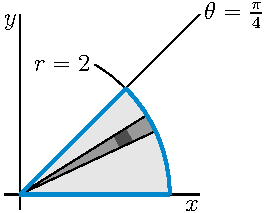
\includegraphics{polar5a2.pdf}\qquad\qquad
     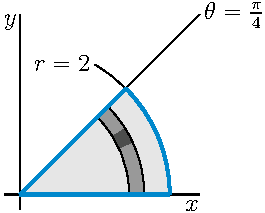
\includegraphics{polar5a3.pdf}
\end{center}
Alternatively, on $\cR$,
\begin{itemize}
\item 
$r$ runs from $0$ to $2$. 
\item
For each fixed $r$ in that range, $\theta$ runs from $0$ to $\frac{\pi}{4}$,
as in the figure on the right above.
\end{itemize}
So 
\begin{equation*}
\dblInt_\cR f(x,y)\,\dee{x}\,\dee{y}
=\int_0^2\dee{r}
  \int_0^{\nicefrac{\pi}{4}}\dee{\theta}
 \ r\ f(r\cos\theta,r\sin\theta)
\end{equation*}


(b) The region 
\begin{equation*}
\cR=\Set{(x,y)}{1\le x^2+y^2\le 4,\ x\ge 0,\ y\ge 0}
\end{equation*}
In polar coordinates, 
\begin{itemize}
\item
the circle $x^2+y^2=1$ becomes $r^2=1$ or $r=1$ and 
\item
the circle $x^2+y^2=4$ becomes $r^2=4$ or $r=2$ and 
\item
the positive $x$-axis, $x\ge0$, $y=0$,  becomes $\theta=0$ and
\item
the positive $y$-axis, $x=0$, $y\ge0$,  becomes $\theta=\frac{\pi}{2}$. 
\end{itemize}
Thus the domain of integration is
\begin{equation*}
\cR=\Set{(r\cos\theta,r\sin\theta)}{1\le r\le 2,\ 0\le\theta\le\tfrac{\pi}{2}}
\end{equation*}
On this domain,
\begin{itemize}
\item 
$\theta$ runs from $0$ to $\frac{\pi}{2}$. 
\item
For each fixed $\theta$ in that range, $r$ runs from $1$ to $2$, 
as in the figure on the left below.
\end{itemize}
In polar coordinates $\dee{x}\,\dee{y} = r\,\dee{r}\,\dee{\theta}$, so that
\begin{equation*}
\dblInt_\cR f(x,y)\,\dee{x}\,\dee{y}
=\int_0^{\nicefrac{\pi}{2}}\dee{\theta}
 \int_1^2\dee{r}\ r\ f(r\cos\theta,r\sin\theta)
\end{equation*}
\begin{center}
     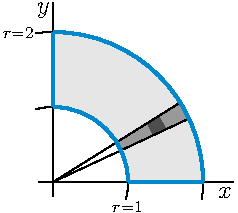
\includegraphics{polar5b2.pdf}\qquad\qquad
     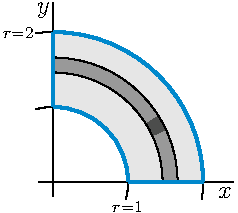
\includegraphics{polar5b3.pdf}
\end{center}
Alternatively, on $\cR$,
\begin{itemize}
\item 
$r$ runs from $1$ to $2$. 
\item
For each fixed $r$ in that range, $\theta$ runs from $0$ to $\frac{\pi}{2}$,
as in the figure on the right above.
\end{itemize}
So 
\begin{equation*}
\dblInt_\cR f(x,y)\,\dee{x}\,\dee{y}
=\int_1^2\dee{r}
  \int_0^{\nicefrac{\pi}{2}}\dee{\theta}
 \ r\ f(r\cos\theta,r\sin\theta)
\end{equation*}

(c) The region 
\begin{equation*}
\cR=\Set{(x,y)}{(x-1)^2+y^2\le 1,\ y \ge 0}
\end{equation*}
In polar coordinates, the circle $(x-1)^2+y^2= 1$, or $x^2-2x+y^2=0$,
is $r^2-2r\cos\theta=0$ or $r=2\cos\theta$. Note that, on $r=2\cos\theta$,
\begin{itemize}
\item
when $\theta=0$, $r=2$ and
\item
as $\theta$ increases from $0$ towards $\nicefrac{\pi}{2}$, $r$ decreases but remains strictly bigger than $0$ (look at the figure below), until
\item
when $\theta=\frac{\pi}{2}$, $r=0$.
\end{itemize}
\begin{center}
     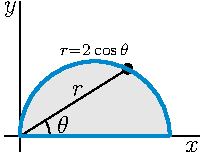
\includegraphics{polar5e4.pdf}
\end{center}
Thus the domain of integration is
\begin{equation*}
\cR=\Set{(r\cos\theta,r\sin\theta)}{0\le\theta\le\tfrac{\pi}{2},\ 
          0\le r\le 2\cos\theta}
\end{equation*}
On this domain,
\begin{itemize}
\item 
$\theta$ runs from $0$ to $\frac{\pi}{2}$. 
\item
For each fixed $\theta$ in that range, $r$ runs from $0$ to $2\cos\theta$, 
as in the figure on the left below.
\end{itemize}
In polar coordinates $\dee{x}\,\dee{y} = r\,\dee{r}\,\dee{\theta}$, so that
\begin{equation*}
\dblInt_\cR f(x,y)\,\dee{x}\,\dee{y}
=\int_0^{\nicefrac{\pi}{2}}\dee{\theta}
 \int_0^{2\cos\theta}\dee{r}\ r\ f(r\cos\theta,r\sin\theta)
\end{equation*}
\begin{center}
     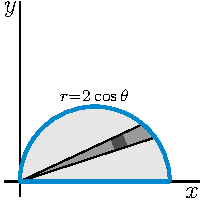
\includegraphics{polar5e2.pdf}\qquad\qquad
     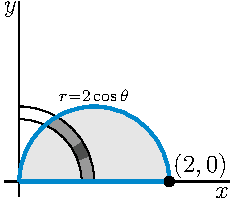
\includegraphics{polar5e3.pdf}
\end{center}
Alternatively, on $\cR$,
\begin{itemize}
\item 
$r$ runs from $0$ (at the point $(0,0)$)  
to $2$ (at the point $(2,0)$). 
\item
For each fixed $r$ in that range, $\theta$ runs 
from $0$ to $\arccos\frac{r}{2}$ (which was gotten by solving 
$r=2\cos\theta$ for $\theta$ as a function of $r$), as in the figure 
on the right above.
\end{itemize}
So 
\begin{equation*}
\dblInt_\cR f(x,y)\,\dee{x}\,\dee{y}
=\int_0^2\dee{r}
  \int_0^{\arccos\frac{r}{2}}\dee{\theta}
 \ r\ f(r\cos\theta,r\sin\theta)
\end{equation*}


(d) The region 
\begin{equation*}
\cR=\Set{(x,y)}{0\le y\le 2,\ 0\le x\le y}
\end{equation*}
In polar coordinates, 
\begin{itemize}
\item
the line $y=2$ becomes $r\sin\theta=2$ and 
\item
the positive $y$-axis, $x=0$, $y\ge0$,  becomes $\theta=\frac{\pi}{2}$ and
\item
the line $y=x$ becomes $r\sin\theta=r\cos\theta$ or $\tan\theta=1$ 
or $\theta=\frac{\pi}{4}$.  
\end{itemize}
Thus the domain of integration is
\begin{equation*}
\cR=\Set{(r\cos\theta,r\sin\theta)}{\tfrac{\pi}{4}\le\theta\le\tfrac{\pi}{2},\ 
          0\le r\sin\theta\le 2}
\end{equation*}
On this domain,
\begin{itemize}
\item 
$\theta$ runs from $\frac{\pi}{4}$ to $\frac{\pi}{2}$. 
\item
For each fixed $\theta$ in that range, $r$ runs from $0$ to 
$\frac{2}{\sin\theta}$, as in the figure on the left below.
\end{itemize}
In polar coordinates $\dee{x}\,\dee{y} = r\,\dee{r}\,\dee{\theta}$, so that
\begin{equation*}
\dblInt_\cR f(x,y)\,\dee{x}\,\dee{y}
=\int_{\nicefrac{\pi}{4}}^{\nicefrac{\pi}{2}}\dee{\theta}
 \int_0^{\nicefrac{2}{\sin\theta}}\dee{r}\ r\ f(r\cos\theta,r\sin\theta)
\end{equation*}
\begin{center}
     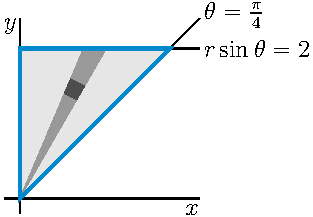
\includegraphics{polar5c2.pdf}\quad
     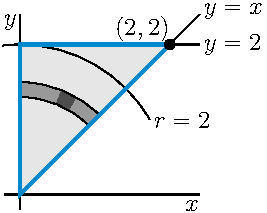
\includegraphics{polar5c4.pdf}\quad
     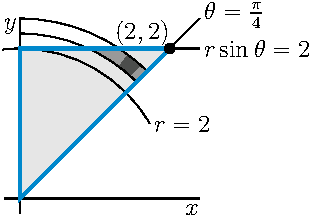
\includegraphics{polar5c5.pdf}
\end{center}
Alternatively, on $\cR$,
\begin{itemize}
\item 
$r$ runs from $0$ (at the point $(0,0)$)  
to $2\sqrt{2}$ (at the point $(2,2)$). 
\item
For each fixed $r$ between $0$ and $2$, $\theta$ runs from $\frac{\pi}{4}$ 
to $\frac{\pi}{2}$, as in the central figure above.
\item
For each fixed $r$ between $2$ and $2\sqrt{2}$, $\theta$ runs 
from $\frac{\pi}{4}$ to $\arcsin\frac{2}{r}$ (which was gotten by solving 
$r\sin\theta=2$ for $\theta$ as a function of $r$), as in the figure 
on the right above.
\end{itemize}
So 
\begin{equation*}
\dblInt_\cR f(x,y)\,\dee{x}\,\dee{y}
=\int_0^2\dee{r}
  \int_{\nicefrac{\pi}{4}}^{\nicefrac{\pi}{2}}\dee{\theta}
 \ r\ f(r\cos\theta,r\sin\theta)
+\int_2^{2\sqrt{2}}\dee{r}
  \int_{\nicefrac{\pi}{4}}^{\arcsin\frac{2}{r}}\dee{\theta}
 \ r\ f(r\cos\theta,r\sin\theta)
\end{equation*}

\end{solution}

%%%%%%%%%%%%%%%%%%%%%%%%%%%%%%%%%%%%%%%%%%%%%%%%%%%%%%%
\begin{question}
Sketch the domain of integration in the $xy$-plane for each of the 
following polar coordinate integrals.
\begin{enumerate}[(a)]
\item
$\displaystyle 
      \int_1^2\dee{r}
     \int_{-\nicefrac{\pi}{4}}^{\nicefrac{\pi}{4}}\dee{\theta}
     \ r\ f(r\cos\theta,r\sin\theta)$

\item
$\displaystyle 
     \int_0^{\nicefrac{\pi}{4}}\dee{\theta}
     \int_0^{\frac{2}{\sin\theta+\cos\theta}}\dee{r}
     \ r\ f(r\cos\theta,r\sin\theta)$
\item
$\displaystyle 
     \int_0^{2\pi}\dee{\theta}
     \int_0^{\frac{3}{\sqrt{\cos^2\theta+9\sin^2\theta}}}\dee{r}
     \ r\ f(r\cos\theta,r\sin\theta)$
\end{enumerate}
\end{question}

%\begin{hint}
%\end{hint}

\begin{answer}
\begin{center}
    (a)\quad 
     \raisebox{-0.9\height}{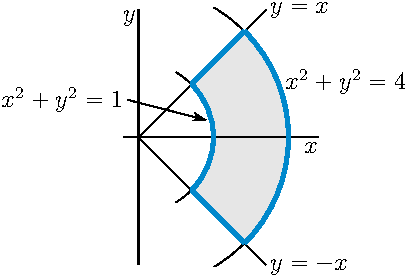
\includegraphics{polar6a2.pdf}}\hfill
    (b)\quad \raisebox{-0.9\height}{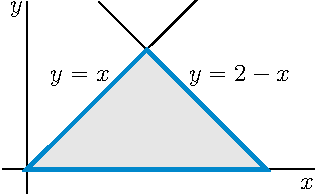
\includegraphics{polar6b2.pdf}}
\end{center}

(c)
\begin{center}
     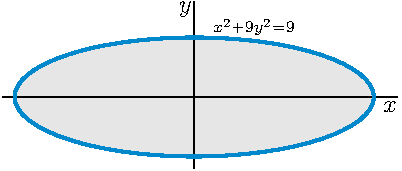
\includegraphics{polar6c2.pdf}
\end{center}

\end{answer}

\begin{solution}
(a)
Let $D$ denote the domain of integration. The symbols
$\displaystyle 
      \int_1^2\dee{r}
     \int_{-\nicefrac{\pi}{4}}^{\nicefrac{\pi}{4}}\dee{\theta}$ 
say that, on $D$,
\begin{itemize}
\item 
$r$ runs from $1$ to $2$ and
\item 
for each $r$ in that range,
$\theta$ runs from $-\frac{\pi}{4}$ to $\frac{\pi}{4}$.
\end{itemize}
In Cartesian coordinates
\begin{itemize}
\item 
$r=1$ is the circle $x^2+y^2=1$ and
\item 
$r=2$ is the circle $x^2+y^2=4$ and
\item
$\theta=\frac{\pi}{4}$ is the ray $y=x$, $x\ge 0$ and
\item 
$\theta=-\frac{\pi}{4}$ is the ray $y=-x$, $x\ge 0$.

\end{itemize}
So
\begin{align*}
D=\Set{(x,y)}{1\le x^2+y^2\le 4,\ -x\le y\le x,\ x\ge 0}
\end{align*}
Here are two sketches. $D$ is the shaded region in the sketch on the right.
\begin{center}
     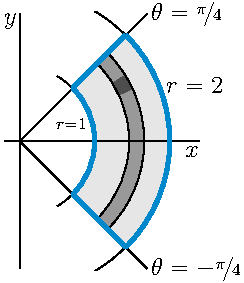
\includegraphics{polar6a1.pdf}\quad
     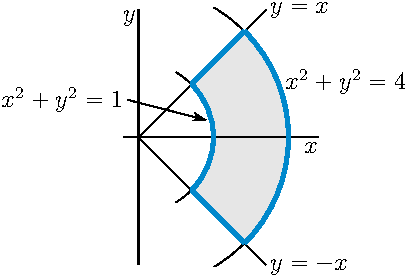
\includegraphics{polar6a2.pdf}
\end{center}

(b)
Let $D$ denote the domain of integration. The symbols
$\int_0^{\nicefrac{\pi}{4}}\dee{\theta}
     \int_0^{\frac{2}{\sin\theta+\cos\theta}}\dee{r}$ 
say that, on $D$,
\begin{itemize}
\item 
$\theta$ runs from $0$ to $\nicefrac{\pi}{4}$ and
\item 
for each $\theta$ in that range,
$r$ runs from $0$ to $\frac{2}{\sin\theta+\cos\theta}$.
\end{itemize}
In Cartesian coordinates
\begin{itemize}
\item 
$\theta=0$ is the positive $x$-axis and
\item
$\theta=\nicefrac{\pi}{4}$ is the ray $y=x$, $x\ge 0$ and
\item 
$r=\frac{2}{\sin\theta+\cos\theta}$, or equivalently
$r\cos\theta+r\sin\theta=2$, is the line $x+y=2$.
\end{itemize}
Looking at the sketch on the left below, we see that,
since the lines $y=x$ and $x+y=2$ cross at $(1,1)$,
\begin{align*}
D=\Set{(x,y)}{0\le y\le 1,\ y\le x\le 2-y}
\end{align*}
$D$ is the shaded region in the sketch on the right.
\begin{center}
     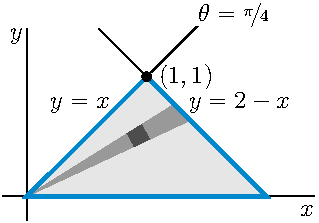
\includegraphics{polar6b1.pdf}\qquad\qquad
     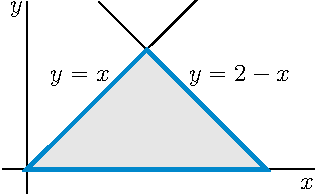
\includegraphics{polar6b2.pdf}
\end{center}


(c)
Let $D$ denote the domain of integration. The symbols
$\int_0^{2\pi}\dee{\theta}
     \int_0^{\frac{3}{\sqrt{\cos^2\theta+9\sin^2\theta}}}\dee{r}$ 
say that, on $D$,
\begin{itemize}
\item 
$\theta$ runs all the way from $0$ to $2\pi$ and
\item 
for each $\theta$,
$r$ runs from $0$ to $\frac{3}{\sqrt{\cos^2\theta+9\sin^2\theta}}$.
\end{itemize}
In Cartesian coordinates
\begin{itemize}
\item 
$r=\frac{3}{\sqrt{\cos^2\theta+9\sin^2\theta}}$, or equivalently
$r^2\cos^2\theta+9r^2\sin^2\theta=9$, is the ellipse $x^2+9y^2=9$.
\end{itemize}
So $D$ is the interior of the ellipse $x^2+9y^2=9$
and $D$ is the shaded region in the sketch on the right.
\begin{center}
     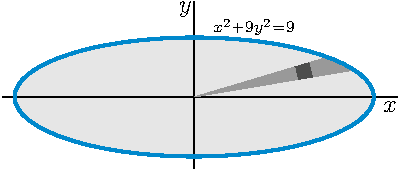
\includegraphics{polar6c1.pdf}\qquad\qquad
     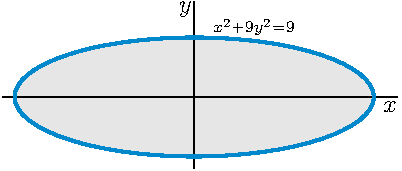
\includegraphics{polar6c2.pdf}
\end{center}

\end{solution}



%%%%%%%%%%%%%%%%%%
\subsection*{\Procedural}
%%%%%%%%%%%%%%%%%%

%%%%%%%%%%%%%%%%%%%%%%%%%%%%%%%%
\begin{question}
Use polar coordinates to evaluate each of the following integrals.
\begin{enumerate}[(a)]
\item
$\displaystyle\dblInt_S (x+y)\dee{x}\,\dee{y}$ where $S$ is the region 
in the first quadrant lying inside the disc $x^2+y^2\le a^2$ and under 
the line $y=\sqrt{3}x$.
\item 
$\displaystyle\dblInt_Sx\ \dee{x}\,\dee{y}$, where $S$  is the disc segment
$x^2+y^2\le 2,\ x\ge 1$.
\item
$\displaystyle\dblInt_T (x^2+y^2)\dee{x}\,\dee{y}$ where $T$ is the triangle
with vertices $(0,0), (1,0)$ and $(1,1)$.
\item
$\displaystyle\dblInt_{x^2+y^2\le 1} \ln(x^2+y^2)\,\dee{x}\,\dee{y}$
\end{enumerate}
\end{question}

%\begin{hint}
%
%\end{hint}

\begin{answer}
(a) $\frac{a^3}{6}\big[\sqrt{3}+1\big]$\qquad
(b) $\frac{2}{3}$  \qquad
(c) $\frac{1}{3}$ \qquad
(d) $-\pi$
\end{answer}

\begin{solution}
(a) In polar coordinates, the domain of integration,
$x^2+y^2\le a^2$, $0\le y\le \sqrt{3}x$, becomes 
\begin{equation*}
0\le r\le a,\ 0\le r\sin\theta\le\sqrt{3}r\cos\theta\qquad\text{ or }\qquad
0\le r\le a,\ 0\le\theta\le \arctan\sqrt{3}=\frac{\pi}{3}
\end{equation*}
The integral is 
\begin{align*}
\dblInt_S (x+y)\dee{x}\,\dee{y}
&=\int_0^a \dee{r}\int_0^{{\pi\over 3}}\dee{\theta}\ r\,(r\cos\theta+r\sin\theta)\\
&=\int_0^a \dee{r}\ r^2\Big[\sin\theta-\cos\theta\Big]_0^{{\pi\over 3}}
=\frac{a^3}{3}\left[\frac{\sqrt{3}}{2}-\frac{1}{2}+1\right]
=\frac{a^3}{6}\big[\sqrt{3}+1\big]
\end{align*}

(b) 
In polar coordinates, the domain of integration,
$x^2+y^2\le 2$, $x\ge 1$, 

\begin{center}
     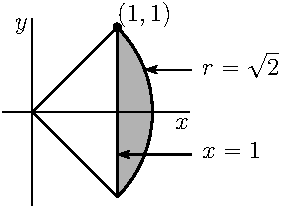
\includegraphics{domain1b.pdf}
\end{center}

becomes 
\begin{equation*}
r\le \sqrt{2},\ r\cos\theta\ge 1\qquad\text{ or }\qquad
  \frac{1}{\cos\theta}\le r\le\sqrt{2}
%%%%%%%%%%%%%%%%%%%%%%\qquad\figplace{domain1b}{0 in}{-0.5 in}
\end{equation*}
For $\frac{1}{\cos\theta}\le r\le\sqrt{2}$ to be nonempty, we need
$\cos\theta\le \frac{1}{\sqrt{2}}$ or $|\theta|\le\frac{\pi}{4}$.
By symmetry under $y\rightarrow -y$, the integral is 
\begin{align*}
\dblInt_Sx\ \dee{x}\,\dee{y}
&=2\int_0^{{\pi\over 4}}\dee{\theta}\int_{1\over\cos\theta}^{\sqrt{2}} 
\dee{r}\ r\,(r\cos\theta)\\
&=2\int_0^{{\pi\over 4}}\dee{\theta}\ \cos\theta\ 
\frac{r^3}{3}\bigg|_{1\over\cos\theta}^{\sqrt{2}} 
=\frac{2}{3}\int_0^{{\pi\over 4}}\dee{\theta}\ 
\Big[2^{3/2}\cos\theta-\frac{1}{\cos^2\theta}\Big] \\
&=\frac{2}{3} \Big[2^{3/2}\sin\theta-\tan\theta\Big]_0^{{\pi\over 4}}
=\frac{2}{3} \big[2^{3/2}\frac{1}{\sqrt{2}}-1\big]
=\frac{2}{3}
\end{align*}

(c) In polar coordinates, the triangle
with vertices $(0,0), (1,0)$ and $(1,1)$ has sides $\theta=0$, 
$\theta=\frac{\pi}{4}$ and $r=\frac{1}{\cos\theta}$ (which is the polar 
coordinates version of $x=1$). The integral is 
\begin{align*}
\dblInt_T (x^2+y^2)\ \dee{x}\,\dee{y}
&=\int_0^{{\pi\over 4}}\dee{\theta}\int_0^{1\over\cos\theta} 
                                                  \dee{r}\ r(r^2)\\
&=\int_0^{{\pi\over 4}}\dee{\theta}\ 
\frac{r^4}{4}\bigg|_0^{1\over\cos\theta}  
=\frac{1}{4}\int_0^{{\pi\over 4}}\dee{\theta}\ \frac{1}{\cos^4\theta}
=\frac{1}{4}\int_0^{{\pi\over 4}}\dee{\theta}\ \sec^4\theta\cr
&=\frac{1}{4}\int_0^{{\pi\over 4}}\dee{\theta}\ \sec^2\theta\big(1+\tan^2\theta\big)
=\frac{1}{4}\int_0^1d t\ \big(1+t^2\big)\text{ where $t=\tan\theta$ }\cr
&=\frac{1}{4}\left[t+\frac{t^3}{3}\right]_0^1
=\frac{1}{4}\ \frac{4}{3}
=\frac{1}{3}
\end{align*}

(d) In polar coordinates, the domain of integration,
$x^2+y^2\le 1$, becomes $0\le r\le 1$, $0\le\theta\le 2\pi$. So
\begin{align*}
\dblInt_{x^2+y^2\le 1}\hskip-5pt \ln(x^2+y^2)\,\dee{x}\,\dee{y}
&=\int_0^{2\pi}\hskip-3pt \dee{\theta}\int_0^1\dee{r}\ r\ln r^2
=2\pi\int_0^1\dee{r}\ r\ln r^2
=\pi\int_0^1 \dee{s}\ \ln s\text{ where $s=r^2$ }\cr
&=\pi\Big[s\ln s-s\Big]_0^1
=-\pi
\end{align*}
To be picky, $\ln s$ tends to $-\infty$ as $s$ tends to $0$.
So $\int_0^1\dee{s}\,\ln s$ is an improper integral. The careful way to
evaluate it is
\begin{align*}
\int_0^1 \dee{s}\ \ln s
&=\lim_{\veps\to 0^+}\int_\veps^1 \dee{s}\ \ln s
=\lim_{\veps\to 0^+}\Big[s\ln s-s\Big]_\veps^1
=\lim_{\veps\to 0^+}\Big[-1-\veps\ln\veps+\veps\Big]
=-1
\end{align*}
That $\lim\limits_{\veps\to 0^+}\veps\ln\veps = 0$ was shown in 
Example \eref{CLP100}{eg:hopitalJ} of the CLP-1 text.


\end{solution}

%%%%%%%%%%%%%%%%%%%%%%%%%%%%%%%%
\begin{question}
Find the volume lying inside the sphere $x^2+y^2+z^2=2$ 
and above the paraboloid $z=x^2+y^2$.
\end{question}

%\begin{hint}
%
%\end{hint}

\begin{answer}
$\pi \left[\frac{4}{3}\sqrt{2}-\frac{7}{6}\right] 
\approx 2.26$
\end{answer}

\begin{solution}
The top surface $x^2+y^2+z^2=2$ meets the bottom surface
$z=x^2+y^2$ when $z$ obeys $x^2+y^2=z=2-z^2$. That is, when 
$0=z^2+z-2=(z-1)(z+2)$. The root $z=-2$ is inconsistent with 
$z=x^2+y^2\ge 0$. So the top and bottom surfaces meet at the circle
$z=1$, $x^2+y^2=1$.

In polar coordinates, the top surface is $z^2=2-r^2$, or equivalently
$z=\sqrt{2-r^2}$, and the bottom surface is $z=r^2$. So the height of the volume
above the point with polar coordinates $(r,\theta)$ is
$\sqrt{2-r^2}-r^2$ and
\begin{align*}
\text{Volume}&=\int_0^1\dee{r}\int_0^{2\pi} \dee{\theta}\ r\,\big[\sqrt{2-r^2}-r^2\big]
=2\pi \int_0^1\dee{r}\ r\,\big[\sqrt{2-r^2}-r^2\big]\\
&=2\pi \left[-\frac{1}{3}{(2-r^2)}^{3/2}-\frac{r^4}{4}\right]_0^1
=2\pi \left[-\frac{1}{3}-\frac{1}{4}+\frac{1}{3}2^{3/2}\right] \\
&=\pi \left[\frac{4}{3}\sqrt{2}-\frac{7}{6}\right] 
\approx 2.26
\end{align*}
In Cartesian coordinates
\begin{align*}
\text{Volume}&=4\int_0^1\dee{x}\int_0^{\sqrt{1-x^2}} \dee{y}\ 
                       \big[\sqrt{2-x^2-y^2}-x^2-y^2\big]
\end{align*}
The $y$ integral can be done using the substitution $y=\sqrt{2-x^2}\cos t$,
but it is easier to use polar coordinates.
\end{solution}

%%%%%%%%%%%%%%%%%%%%%%%%%%%%%%%%
\begin{question}
Let $a>0$.
Find the volume lying inside the cylinder $x^2+(y-a)^2=a^2$ 
and between the upper and lower halves of the cone $z^2=x^2+y^2$.
\end{question}

%\begin{hint}
%
%\end{hint}

\begin{answer}
$\frac{64}{9}a^3$
\end{answer}

\begin{solution}
For this region $x$ and $y$ run over the interior of the 
cylinder $x^2+(y-a)^2=a^2$. For each $(x,y)$ inside the 
cylinder, $z$ runs from $-\sqrt{x^2+y^2}$ to $\sqrt{x^2+y^2}$.
As $x^2+(y-a)^2=a^2$ if and only if $x^2+y^2-2ay=0$, the cylinder
has equation $r^2=2ar\sin\theta$, or equivalently, $r=2a\sin\theta$,
in polar coordinates. 
\vadjust{
\begin{center}
     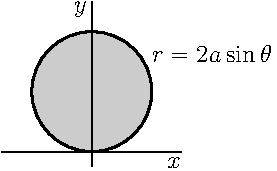
\includegraphics{domain2.pdf}
\end{center}
}%
Thus $(r,\theta)$ runs over $0\le\theta\le\pi,\ 
0\le r\le 2a\sin\theta$ and for each $(r,\theta)$ in this region $z$ runs from
$-r$ to $r$. By symmetry under $x\rightarrow -x$,
the volume is
\begin{align*}
\text{Volume}
&=2\int_0^{{\pi\over 2}}\dee{\theta}\int_0^{2a\sin\theta}\dee{r}\  
                                             r\big[r-(-r)\big]
=4\int_0^{{\pi\over 2}}\dee{\theta}\int_0^{2a\sin\theta}\dee{r}\ r^2
=\frac{4}{3}\int_0^{{\pi\over 2}}\!\!\dee{\theta}\ (2a\sin\theta)^3 \\
&=\frac{32}{3}a^3\int_0^{{\pi\over 2}}\!\!\dee{\theta}\ \sin\theta(1-\cos^2\theta)
=-\frac{32}{3}a^3\int_1^0 dt\ (1-t^2)\text{ where $t=\cos\theta$ }\cr
&=-\frac{32}{3}a^3\left[t-\frac{t^3}{3}\right]_1^0
=\frac{64}{9}a^3
\end{align*}
\end{solution}

%%%%%%%%%%%%%%%%%%%%%%%%%%%%%%%%
\begin{question}
Let $a>0$.
Find the volume common to the cylinders $x^2+y^2\le 2ax$ and 
$z^2\le 2ax$.
\end{question}

%\begin{hint}
%
%\end{hint}

\begin{answer}
$\frac{128}{15}a^3$
\end{answer}

\begin{solution}
The figure below shows the top view of the specified solid.
$(x,y)$ runs over the interior of the circle $x^2+y^2=2ax$. For each fixed
$(x,y)$ in this disk, $z$ runs from $-\sqrt{2ax}$ to $+\sqrt{2ax}$. In polar
coordinates, the circle is $r^2=2ar\cos\theta$ or $r=2a\cos\theta$. 
\vadjust{
\begin{center}
     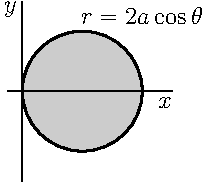
\includegraphics{domainTwoCylinder.pdf}
\end{center}
}%
The solid
is symmetric under $y\rightarrow -y$ and $z\rightarrow -z$, so we can restrict
to $y\ge 0$, $z\ge 0$ and multiply by 4. The volume is
\begin{align*}
\text{Volume}
&=4\int_0^{\pi\over 2} \dee{\theta}\int_0^{2a\cos\theta} \dee{r}\  
                                                r\sqrt{2ar\cos\theta}
\\
&=4\int_0^{\pi\over 2} \dee{\theta}\ \sqrt{2a\cos\theta}\ \frac{2}{5}\ 
                                 r^{5/2}\bigg|_0^{2a\cos\theta}
\\
&=\frac{8}{5}\int_0^{\pi\over 2} \dee{\theta}\ \big(2a\cos\theta\big)^3
=\frac{64}{5}a^3\int_0^{\pi\over 2} \dee{\theta}\ \cos\theta\big(1-\sin^2\theta\big)\cr
&=\frac{64}{5}a^3\int_0^1 dt\ \big(1-t^2\big)
\qquad\text{ where $t=\sin\theta$}\cr
&=\frac{64}{5}a^3\left[t-\frac{t^3}{3}\right]_0^1
=\frac{128}{15}a^3
\end{align*}
\end{solution}


%%%%%%%%%%%%%%%%%%%%%%%%%%%%%%%%
\begin{question}[M200 2005D] %8
Consider  the region $E$ in 3--dimensions specified by the inequalities 
$x^2 + y^2 \le 2y$ and $0 \le z \le \sqrt{x^2 + y^2}$.
\begin{enumerate}[(a)]
\item
  Draw a reasonably accurate picture of $E$ in 3--dimensions. 
Be sure to show the units on the coordinate axes.
\item 
  Use polar coordinates to find the volume of $E$. Note that you will 
  be ``using polar coordinates'' if you solve this problem
 by means of cylindrical coordinates. 

 \emph{Hint:}\ \ \ 
    $\int \sin^n u\ \dee{u} =-\frac{1}{n}\sin^{n-1}u\ \cos u
                 +\frac{n-1}{n}\int\sin^{n-2}u\ \dee{u}$
\end{enumerate}
\end{question}

%\begin{hint}
%
%\end{hint}

\begin{answer}
(a)
\begin{center}
     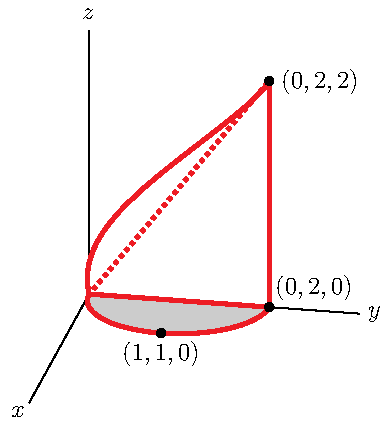
\includegraphics[scale=0.8]{OE05D_8.pdf}
\end{center}

(b) $\frac{32}{9}$
\end{answer}

\begin{solution}
(a) 
\begin{itemize}
\item
The equation $x^2 + y^2 \le 2y$ is equivalent to the
equation $x^2 + (y-1)^2=1$, which is the equation of the cylinder whose
$z=z_0$ cross--section is the horizontal circle of radius $1$, centred on 
$x=0$, $y=1$, $z=z_0$. The part of this cylinder in the first octant is
sketched in the figure on the left below.

\item
$z \le \sqrt{x^2 + y^2}$ is the equation of the cone with vertex $(0,0,0)$,
and axis the positive $z$--axis, whose radius at height $z=2$ is $2$.
The part of this cone in the first octant is sketched in the figure
on the right below.

\end{itemize}

\begin{center}
     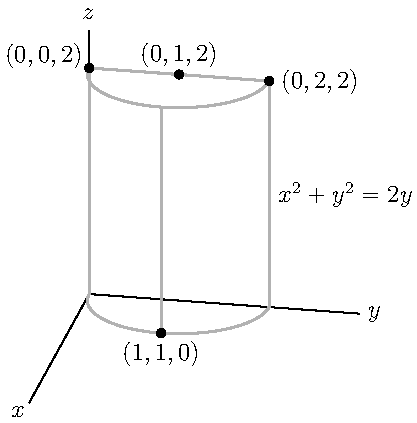
\includegraphics{OE05D_8a.pdf}\quad
     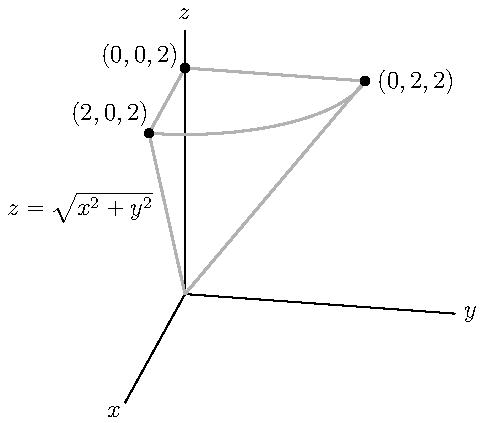
\includegraphics{OE05D_8b.pdf}
\end{center}

The region $E$ is the part of the cylinder that is above the
$xy$--plane (since $z\ge 0$) outside the cone (since $z\le\sqrt{x^2+y^2}$).
The part of $E$ that is in the first octant is outlined in red in the
figure below. Both $x^2 + y^2 \le 2y$ and $0 \le z \le \sqrt{x^2 + y^2}$
are invariant under $x\rightarrow -x$. So $E$ is also invariant
under $x\rightarrow -x$. That is, $E$ is symmetric about the $yz$--plane
and contains, in the octant $x\le 0$, $y\ge 0$, $z\ge 0$, a mirror
image of the first octant part of $E$.

\begin{center}
     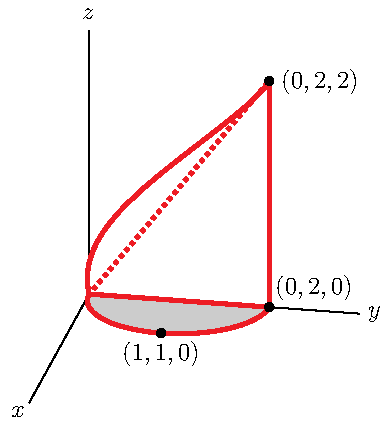
\includegraphics{OE05D_8.pdf}
\end{center}

(b) In polar coordinates, $x^2 + y^2 \le 2y$ becomes
\begin{equation*}
r^2\le 2r\sin\theta 
\iff 
r\le 2\sin\theta
\end{equation*}
Let us denote by $D$ the base region of the part of $E$ in the first 
octant (i.e. the shaded region in the figure above). Think of $D$ as being
part of the $xy$--plane. In polar coordinates, on $D$
\begin{itemize}
\item 
$\theta$ runs from $0$ to $\frac{\pi}{2}$. (Recall that $D$ is 
contained in the first quadrant.)
\item
For each $\theta$ in that range, $r$ runs from $0$ to $2\sin\theta$.
\end{itemize}
Because
\begin{itemize}
\item
in polar coordinates $\dee{A} = r\,\dee{r}\,\dee{\theta}$, and
\item 
the height of $E$ above each point $(x,y)$ in $D$ is $\sqrt{x^2+y^2}$,
or, in polar coordinates, $r$, and
\item 
the volume of $E$ is twice the volume of the part of $E$ in the first octant,
\end{itemize}
we have
\begin{align*}
\text{Volume}(E)
&= 2\int_0^{\frac{\pi}{2}}\dee{\theta} \int_0^{2\sin\theta}\dee{r}\ r^2 \\
&=\frac{16}{3} \int_0^{\frac{\pi}{2}}\dee{\theta}\ \sin^3\theta 
=\frac{16}{3} \int_0^{\frac{\pi}{2}}\dee{\theta}\ 
                  \sin\theta\ \big(1-\cos^2\theta\big) \\
&=-\frac{16}{3} \int_1^0\dee{u}\ \big(1-u^2\big)\qquad
\text{with }u=\cos\theta,\ \dee{u}=-\sin\theta\ \dee{\theta} \\
&=\frac{16}{3}\left[1-\frac{1}{3}\right] \\
&=\frac{32}{9}
\end{align*}
\end{solution}

%%%%%%%%%%%%%%%%%%%%%%%%%%%%%%%%
\begin{question}[M200 2006A] %7
Evaluate the iterated double integral
\begin{equation*}
\int_{x=0}^{x=2}\int_{y=0}^{y=\sqrt{4-x^2}} {(x^2+y^2)}^{\frac{3}{2}}\ \dee{y}\,\dee{x}
\end{equation*}
\end{question}

%\begin{hint}
%
%\end{hint}

\begin{answer}
$\frac{16\pi}{5}$
\end{answer}

\begin{solution}
On the domain of integration
\begin{itemize}
\item
$x$ runs for $0$ to $2$, and

\item
for each fixed $x$ in that range, $y$ runs from $0$ to $\sqrt{4-x^2}$.
The equation $y=\sqrt{4-x^2}$ is equivalent to $x^2+y^2=4$, $y\ge 0$.
\end{itemize}
This domain is sketched in the figure on the left below.
\begin{center}
     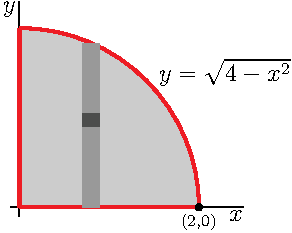
\includegraphics{OE06A_7v.pdf}\qquad
     \includegraphics{OE06A_7p.pdf}
\end{center}
Considering that
\begin{itemize}
\item
the integrand, ${(x^2+y^2)}^{\frac{3}{2}}$, is invariant under rotations 
about the origin and
\item
the outer curve, $x^2+y^2=4$, is invariant under rotations about the origin \end{itemize}
we'll use polar coordinates. 
In polar coordinates, 
\begin{itemize}
\item
the outer curve, $x^2+y^2=4$, is $r=2$, and
\item 
the integrand, ${(x^2+y^2)}^{\frac{3}{2}}$ is $r^3$, and
\item
$\dee{A}=r\,\dee{r}\,\dee{\theta}$
\end{itemize}
Looking at the figure on the right above, we see that the given integral
is, in polar coordinates,
\begin{align*}
\int_0^{\pi/2}\dee{\theta}\int_0^2\dee{r}\ r (r^3)
&=\frac{\pi}{2}\ \frac{2^5}{5}
=\frac{16\pi}{5}
\end{align*}
\end{solution}


%%%%%%%%%%%%%%%%%%%%%%%%%%%%%%%%
\begin{question}[M200 2006D] %5
\begin{enumerate}[(a)]
\item
Sketch the region $\cL$ (in the first quadrant of the $xy$--plane) 
with boundary curves
\begin{equation*}
x^2 + y^2 = 2,\ 
x^2 + y^2 = 4,\ 
y = x,\ 
y = 0.
\end{equation*}
The mass of a thin lamina with a density function $\rho(x,y)$ over 
the region $\cL$ is given by
\begin{equation*}
M =\dblInt_\cL \rho(x,y)\,\dee{A}
\end{equation*}

\item
Find an expression for $M$ as an integral in polar coordinates.

\item
Find M when
\begin{equation*}
\rho(x,y) = \frac{2xy}{x^2+y^2}
\end{equation*}
\end{enumerate}
\end{question}

%\begin{hint}
%
%\end{hint}

\begin{answer}
(a)

\begin{center}
     \includegraphics{OE06D_5.pdf}
\end{center}

(b) $M = \int_0^{\pi/4}\dee{\theta}\int_{\sqrt{2}}^2\dee{r}\ r\,
         \rho(r\cos\theta\,,\,r\sin\theta)$ \qquad
(c) $\frac{1}{2}$
\end{answer}

\begin{solution}
(a) The region $\cL$ is sketched in the figure on the leflt below.
\begin{center}
     \includegraphics{OE06D_5.pdf}\qquad
     \includegraphics{OE06D_5p.pdf}
\end{center}

(b) In polar coordinates
\begin{itemize}
\item
the circle $x^2+y^2=2$ is $r^2=2$ or $r=\sqrt{2}$, and
\item
the circle $x^2+y^2=4$ is $r^2=4$ or $r=2$, and
\item
the line $y=x$ is $r\sin\theta = r\cos\theta$, or $\tan\theta =1 $,
or (for the part in the first quadrant) $\theta=\frac{\pi}{4}$, and
\item 
the positive $x$--axis ($y=0$, $x\ge 0$) is $\theta=0$ 
\end{itemize}
Looking at the figure on the right above, we see that, in $\cL$,
\begin{itemize}
\item 
$\theta$ runs from $0$ to $\frac{\pi}{4}$, and
\item
for each fixed $\theta$ in that range, $r$ runs from $\sqrt{2}$
to $2$.
\item
$\dee{A}$ is $r\,\dee{r}\,\dee{\theta}$
\end{itemize}
So
\begin{align*}
M = \int_0^{\pi/4}\dee{\theta}\int_{\sqrt{2}}^2\dee{r}\ r\,
         \rho(r\cos\theta\,,\,r\sin\theta)
\end{align*}

(c) When
\begin{align*}
\rho = \frac{2xy}{x^2+y^2} = \frac{2r^2\cos\theta\,\sin\theta}{r^2}
     =\sin(2\theta)
\end{align*}
we have
\begin{align*}
M &= \int_0^{\pi/4}\dee{\theta}\int_{\sqrt{2}}^2\dee{r}\ r\,
          \sin(2\theta) \\
&=\left[\int_0^{\pi/4}\sin(2\theta)\ \dee{\theta}\right]
 \left[\int_{\sqrt{2}}^2 r\ \dee{r}\right] \\
&=\left[-\frac{1}{2}\cos(2\theta)\right]_0^{\pi/4}
 \left[ \frac{r^2}{2}\right]_{\sqrt{2}}^2 
  =\frac{1}{2}\ \frac{4-2}{2} \\
&=\frac{1}{2}
\end{align*}
\end{solution}

%%%%%%%%%%%%%%%%%%%%%%%%%%%%%%%%
\begin{question}[M200 2009A] %6
Evaluate $\displaystyle \dblInt_{\bbbr^2} \frac{1}{{(1+x^2+y^2)}^2}\ \dee{A}$.
\end{question}

%\begin{hint}
%
%\end{hint}

\begin{answer}
$\pi$
\end{answer}

\begin{solution}
We'll use polar coordinates. The domain of integration is
\begin{equation*}
\bbbr^2=\Set{(r\cos\theta\,,\,r\sin\theta)}{0\le r<\infty,\ 
                       0\le\theta\le 2\pi}
\end{equation*}
The given integral is improper, so we'll start by integrating $r$ from $0$
to an arbitrary $R>0$, and then we'll take the limit $R\rightarrow\infty$.
In polar coordinates, the integrand
$\frac{1}{{(1+x^2+y^2)}^2}=\frac{1}{{(1+r^2)}^2}$, and
 $\dee{A}=r\,\dee{r}\,\dee{\theta}$, so
\begin{align*}
\dblInt_{\bbbr^2} \frac{1}{{(1+x^2+y^2)}^2}\ \dee{A}
&=\lim_{R\rightarrow\infty} \int_0^{2\pi}\dee{\theta}\int_0^R\dee{r}
                  \frac{r}{{(1+r^2)}^2} \\
&=\lim_{R\rightarrow\infty} \int_0^{2\pi}\dee{\theta}\ 
                      \left[-\frac{1}{2(1+r^2)}\right]_0^R \\
&=\lim_{R\rightarrow\infty} 2\pi
                      \left[\frac{1}{2}-\frac{1}{2(1+R^2)}\right] \\
&=\pi
\end{align*}
\end{solution}

%%%%%%%%%%%%%%%%%%%%%%%%%%%%%%%%
\begin{question}[M200 2011D] %5b
Evaluate the double integral
\begin{equation*}
\dblInt_D y\sqrt{x^2+y^2}\,\dee{A}
\end{equation*}
over the region
$D =\Set{(x,y)}{ x^2+y^2\le 2,\ 0\le y\le x}$.
\end{question}

%\begin{hint}
%
%\end{hint}

\begin{answer}
$1-\frac{1}{\sqrt{2}}$
\end{answer}

\begin{solution}
 Let's switch to polar coordinates. In polar coordinates,
the circle $x^2+y^2=2$ is $r=\sqrt{2}$ and the line $y=x$ is
$\theta=\frac{\pi}{4}$.
\begin{center}
     \includegraphics{OE11D_5bb.pdf}\qquad
\end{center}
In polar coordinates $\dee{A} = r\,\dee{r}\,\dee{\theta}$, so the integral
\begin{align*}
\dblInt_D y\sqrt{x^2+y^2}\,\dee{A}
&=\int_0^{\pi/4}\dee{\theta}\int_0^{\sqrt{2}}\dee{r}\ r\  
 \overbrace{r\sin\theta}^{y}\ \overbrace{r}^{\sqrt{x^2+y^2}} \\
&=\int_0^{\pi/4}\dee{\theta}\ \sin\theta\ 
     \left[\frac{r^4}{4}\right]_0^{\sqrt{2}} \\
&=\Big[-\cos\theta\Big]_0^{\pi/4} \\
&= 1-\frac{1}{\sqrt{2}}
\end{align*}
\end{solution}

\begin{question}[M200 2013D] %5
This question is about the integral
\begin{equation*}
\int_0^1 \int_{\sqrt{3}y}^{\sqrt{4-y^2}} \ln\big(1+x^2+y^2)\
                         \dee{x}\,\dee{y}
\end{equation*}
\begin{enumerate}[(a)]
\item
Sketch the domain of integration.
\item
Evaluate the integral by transforming to polar coordinates.
\end{enumerate}
\end{question}

%\begin{hint}
%
%\end{hint}

\begin{answer}
(a)
\begin{center}
     \includegraphics{OE13D_5a.pdf}
\end{center}

(b) $\frac{\pi}{12}\big[5\ln(5)-4\big]$
\end{answer}

\begin{solution}
(a) On the domain of integration 
\begin{itemize}
\item
$y$ runs from $0$ to $1$. In inequalities, $0\le y\le 1$.
\item
For each fixed $y$ in that range, $x$ runs from $\sqrt{3}\,y$ to
$\sqrt{4-y^2}$. In inequalities, that is $\sqrt{3}\,y\le x\le \sqrt{4-y^2}$.
Note that the inequalities $x\le \sqrt{4-y^2}$, $x\ge 0$ are equivalent to
$x^2+y^2\le 4$, $x\ge 0$.
\end{itemize}
Note that the line $x=\sqrt{3}\, y$ and the circle $x^2+y^2\le 4$
intersect when $3y^2+y^2=4$, i.e. $y=\pm 1$.
Here is a sketch.

\begin{center}
     \includegraphics{OE13D_5.pdf}
\end{center}

(b)
In polar coordinates, the circle $x^2+y^2= 4$ is $r=2$ and the
line $x=\sqrt{3}\, y$, i.e. $\frac{y}{x} =\frac{1}{\sqrt{3}}$, 
is $\tan\theta=\frac{1}{\sqrt{3}}$ or $\theta=\frac{\pi}{6}$.
As $\dee{x}\,\dee{y} = r\,\dee{r}\,\dee{\theta}$,
the domain of integration is
\begin{align*}
\Set{(r\cos\theta,r\sin\theta)}{0\le \theta\le\nicefrac{\pi}{6},\ 0\le r\le 2}
\end{align*}
and
\begin{align*}
\int_0^1 \int_{\sqrt{3}y}^{\sqrt{4-y^2}} \ln\big(1+x^2+y^2)\
                         \dee{x}\,\dee{y}
&= \int_0^2\dee{r}\int_0^{\pi/6}\dee{\theta}\ r\,\ln(1+r^2)
= \frac{\pi}{6}\int_0^2\dee{r}\ r\,\ln(1+r^2) \\
&=\frac{\pi}{12}\int_1^5 \dee{u} \ln(u)
        \qquad\text{with }u=1+r^2,\ \dee{u}=2r\,\dee{r} \\
&=\frac{\pi}{12}\Big[u\ln(u)-u\Big]_1^5 \\
&=\frac{\pi}{12}\big[5\ln(5)-4\big]
\end{align*}
\end{solution}

\begin{question}[M200 2014A] %5
Let $D$ be the region in the $xy$--plane bounded on the left by the line 
$x = 2$ and on the right by the circle $x^2 + y^2 = 16$. Evaluate
\begin{equation*}
\dblInt_D\big(x^2+y^2\big)^{-3/2}\ \dee{A}
\end{equation*}
\end{question}

%\begin{hint}
%
%\end{hint}

\begin{answer}
$\frac{\sqrt{3}}{2}-\frac{\pi}{6}$
\end{answer}

\begin{solution}
Here is a sketch of $D$.

\begin{center}
     \includegraphics{OE14A_5.pdf}
\end{center}

We'll use polar coordinates. In polar coordinates the circle $x^2+y^2=16$
is $r=4$ and the line $x=2$ is $r\cos\theta =2$. So
\begin{align*}
D = \left\{(r\cos\theta\,,\,r\sin\theta)\ \left|\ 
           -\frac{\pi}{3}\le\theta\le\frac{\pi}{3},\ 
           \frac{2}{\cos\theta}\le r\le 4\ \right.\right\}
\end{align*}
and, as $\dee{A} = r\,\dee{r}\,\dee{\theta}$, the specified integral is
\begin{align*}
\dblInt_D\big(x^2+y^2\big)^{-3/2}\ \dee{A}
&= \int_{-\pi/3}^{\pi/3} \dee{\theta}\int_{2/\cos\theta}^4\dee{r}\ 
           r\frac{1}{r^3} \\
&= \int_{-\pi/3}^{\pi/3} \dee{\theta}\ 
           \left[-\frac{1}{r}\right]_{2/\cos\theta}^4 \\
&= \int_{-\pi/3}^{\pi/3} \dee{\theta}\ 
           \left[\frac{\cos\theta}{2}-\frac{1}{4}\right] \\
&=  \left[\frac{\sin\theta}{2}-\frac{\theta}{4}\right]_{-\pi/3}^{\pi/3} \\
&=\frac{\sqrt{3}}{2}-\frac{\pi}{6}
\end{align*}
\end{solution}

\begin{question}[M200 2014D] %6
In the $xy$--plane, the disk $x^2 + y^2 \le 2x$ is cut into $2$ pieces 
by the line $y = x$. Let $D$ be the larger piece.
\begin{enumerate}[(a)]
\item
Sketch $D$ including an accurate description of the center and radius 
of the given disk. Then describe $D$ in polar coordinates $(r, \theta)$.
\item
Find the volume of the solid below $z = \sqrt{x^2 + y^2}$ and above $D$.
\end{enumerate}
\end{question}

%\begin{hint}
%
%\end{hint}

\begin{answer}
(a) $D = \Set{(r\cos\theta\,,\,r\sin\theta)}
     {-\nicefrac{\pi}{2}\le\theta\le\nicefrac{\pi}{4},\ 0\le r\le 2\cos\theta}$

(b) $\text{Volume}=\frac{40}{18\sqrt{2}} +\frac{16}{9}$
\end{answer}

\begin{solution}
(a) The inequality $x^2 + y^2 \le 2x$ is equivalent to
$(x-1)^2 + y^2 \le 1$ and says that $(x,y)$ is to be inside the disk of
radius $1$ centred on $(1,0)$. Here is a sketch.

\begin{center}
\includegraphics{OE14D_6.pdf}
\end{center}

In polar coordinates, $x=r\cos\theta$, $y=r\sin\theta$ so that 
the line $y=x$ is $\theta=\frac{\pi}{4}$
and the circle $x^2+y^2=2x$ is
\begin{equation*}
r^2=2r\cos\theta \qquad\text{or}\qquad r=2\cos\theta
\end{equation*}
Consequently
\begin{equation*}
D = \Set{(r\cos\theta\,,\,r\sin\theta)}
     {-\nicefrac{\pi}{2}\le\theta\le\nicefrac{\pi}{4},\ 0\le r\le 2\cos\theta}
\end{equation*}

(b) The solid has height $z=r$ above the point in $D$ with polar coordinates
     $r$, $\theta$. So the 
\begin{align*}
\text{Volume}
&= \dblInt_D r\ \dee{A}=\dblInt_D r^2\ \dee{r}\, \dee{\theta}
=\int_{-\pi/2}^{\pi/4}\dee{\theta}\int_0^{2\cos\theta} \dee{r}\ r^2 \\
&= \frac{8}{3}\int_{-\pi/2}^{\pi/4}\dee{\theta}\ \cos^3\theta
= \frac{8}{3}\int_{-\pi/2}^{\pi/4}\dee{\theta}\ 
                         \cos\theta\big[1-\sin^2\theta\big] \\
&=\frac{8}{3} \left[\sin\theta -\frac{\sin^3\theta}{3}\right]_{-\pi/2}^{\pi/4}\\
&=\frac{8}{3}\left[\left(\frac{1}{\sqrt{2}} -\frac{1}{6\sqrt{2}}\right)
                   -\left(-1 + \frac{1}{3}\right)  \right] \\
&=\frac{40}{18\sqrt{2}} +\frac{16}{9}
\end{align*}
\end{solution}

%%%%%%%%%%%%%%%%%%%%%%%%%%%%%%%%
\begin{question}[M200 2000A] %8
Let $D$ be the shaded region in the diagram. Find the average 
distance of points in $D$ from the origin. You may use that
$\int\cos^n(x)\,dx = \frac{\cos^{n-1}(x)\sin(x)}{n}
                        +\frac{n-1}{n}\int\cos^{n-2}(x)\,dx$
for all natural numbers $n\ge 2$.
\begin{center}
     \includegraphics{OE00AQ8.pdf}
\end{center}
\end{question}

%\begin{hint}
%
%\end{hint}

\begin{answer}
$2\frac{\pi+44/9}{\pi+8}\approx 1.442$
\end{answer}

\begin{solution} 
We'll use polar coordinates. In $D$
\begin{itemize}
\item
$\theta$ runs from $0$ to $\frac{\pi}{2}$ and
\item
for each fixed $\theta$ between $0$ and $\frac{\pi}{2}$, $r$ runs from
$1$ to $1+\cos(\theta)$.
\end{itemize}
So the area of $D$ is 
\begin{equation*}
\text{area}=A=\int_0^{\pi/2} \dee{\theta}\int_1^{1+\cos\theta} \dee{r}\ r
=\int_0^{\pi/2} \dee{\theta}\ \frac{1}{2} r^2\bigg|_1^{1+\cos\theta} 
=\int_0^{\pi/2} \dee{\theta}\ \left[\frac{1}{2} \cos^2\theta+\cos\theta\right]
\end{equation*}
We are interested in the average value of $r$ on $D$, which is
\begin{align*}
\text{ave\ dist}&=\frac{1}{A}\int_0^{\pi/2} \dee{\theta}\int_1^{1+\cos\theta} 
                                    \dee{r}\ r^2
=\frac{1}{A}\int_0^{\pi/2} \dee{\theta}\ \frac{1}{3} r^3\bigg|_1^{1+\cos\theta}
\\ 
&=\frac{1}{A}\int_0^{\pi/2} \dee{\theta}\ \left[\frac{1}{3} \cos^3\theta
                +\cos^2\theta+\cos\theta\right] 
\end{align*}
Now we evaluate the integrals of the various powers of cosine.
\begin{align*}
\int_0^{\pi/2}\cos\theta\ \dee{\theta}&=\sin\theta\,\bigg|_0^{\pi/2}=1 \\
\int_0^{\pi/2}\cos^2\theta\ \dee{\theta}&=\frac{\cos\theta\sin\theta}{2}\,\bigg|_0^{\pi/2}
+\frac{1}{2}\int _0^{\pi/2}\dee{\theta}=\frac{\pi}{4}\cr
\int_0^{\pi/2}\cos^3\theta\ \dee{\theta}&=\frac{\cos^2\theta\sin\theta}{3}\,\bigg|_0^{\pi/2}
+\frac{2}{3}\int _0^{\pi/2}\cos\theta\ \dee{\theta}=\frac{2}{3}\cr
\end{align*}
So $A=\frac{\pi}{8}+1$ and
\begin{align*}
\text{ave\ dist}=\frac{8}{\pi+8}\left[\frac{2}{9}+\frac{\pi}{4}+1\right]
=2\frac{\pi+44/9}{\pi+8}\approx 1.442
\end{align*}
\end{solution}



%%%%%%%%%%%%%%%%%%
\subsection*{\Application}
%%%%%%%%%%%%%%%%%%
%%%%%%%%%%%%%%%%%%%%%%%%%%%%%%%%
\begin{question}[M200 2010A] %5
Let $G$ be the region in $\bbbr^2$ given by
\begin{gather*}
x^2 + y^2 \le 1 \\
0 \le x \le 2y \\
y \le 2x
\end{gather*}
\begin{enumerate}[(a)]
\item
Sketch the region $G$.
\item
Express the integral $\dblInt_G f(x,y)\ \dee{A}$ 
a sum of iterated integrals $\dblInt f(x, y)\ \dee{x}\dee{y}$.
\item
Express the integral $\dblInt_G f(x,y)\ \dee{A}$ 
as an iterated integral in polar coordinates $(r, \theta)$ where $x = r \cos(\theta)$ and 
$y = r \sin(\theta)$.
\end{enumerate}
\end{question}

%\begin{hint}
%
%\end{hint}

\begin{answer}
(a)
\begin{center}
     \includegraphics{OE10A_5.pdf}
\end{center}

(b)
\begin{align*}
\dblInt_G f(x,y)\ \dee{A}
&=\int_0^{\frac{1}{\sqrt{5}}}\dee{y}\int_{y/2}^{2y}\dee{x}\ f(x,y)
 +\int_{\frac{1}{\sqrt{5}}}^{\frac{2}{\sqrt{5}}}\dee{y}\int_{y/2}^{\sqrt{1-y^2}}
         \dee{x}\ f(x,y)
\end{align*}

(c)
\begin{align*}
\dblInt_G f(x,y)\ \dee{A}
&=\int_{\arctan\frac{1}{2}}^{\arctan 2}\dee{\theta}
       \int_0^1\dee{r}\ r\,f(r\cos\theta,r\sin\theta)
\end{align*}
\end{answer}

\begin{solution}
(a) Observe that
\begin{itemize}
\item
the condition $x^2+y^2\le 1$ restricts $G$ to the interior of the 
circle of radius $1$ centred on the origin, and
\item
the conditions $0\le x\le 2y$ restricts $G$ to $x\ge 0$, $y\ge 0$,
i.e. to the first quadrant, and
\item
the conditions $x\le 2y$ and $y\le 2x$ restrict $\frac{x}{2}\le y\le 2x$.
So $G$ lies below the (steep) line $y=2x$ and lies above the (not steep)
line $y=\frac{x}{2}$. 
\end{itemize}
Here is a sketch of $G$

\begin{center}
     \includegraphics{OE10A_5.pdf}
\end{center}

(b) Observe that the line $y=2x$ crosses the circle $x^2+y^2=1$ at
a point $(x,y)$ obeying
\begin{align*}
x^2+(2x)^2=x^2+y^2=1
\implies 5x^2=1
\end{align*}
and that the line $x=2y$ crosses the circle $x^2+y^2=1$ at
a point $(x,y)$ obeying
\begin{align*}
(2y)^2+y^2=x^2+y^2=1
\implies 5y^2=1
\end{align*}
So the intersection point of $y=2x$ and $x^2+y^2=1$ in the first octant
is $\left(\frac{1}{\sqrt{5}}\,,\,\frac{2}{\sqrt{5}}\right)$ and 
the intersection point of $x=2y$ and $x^2+y^2=1$ in the first octant
is $\left(\frac{2}{\sqrt{5}}\,,\,\frac{1}{\sqrt{5}}\right)$.

We'll set up the iterated integral using horizontal strips as in the
sketch
\begin{center}
     \includegraphics{OE10A_5xy.pdf}
\end{center}

Looking at that sketch, we see that, on $G$,
\begin{itemize}
\item
$y$ runs from $0$ to $\frac{2}{\sqrt{5}}$, and
\item
for each fixed $y$ between $0$ and $\frac{1}{\sqrt{5}}$,
$x$ runs from $\frac{y}{2}$ to $2y$, and
\item
for each fixed $y$ between $\frac{1}{\sqrt{5}}$ and $\frac{2}{\sqrt{5}}$
$x$ runs from $\frac{y}{2}$ to $\sqrt{1-y^2}$.
\end{itemize}
So
\begin{align*}
\dblInt_G f(x,y)\ \dee{A}
&=\int_0^{\frac{1}{\sqrt{5}}}\dee{y}\int_{y/2}^{2y}\dee{x}\ f(x,y)
 +\int_{\frac{1}{\sqrt{5}}}^{\frac{2}{\sqrt{5}}}\dee{y}\int_{y/2}^{\sqrt{1-y^2}}
         \dee{x}\ f(x,y)
\end{align*}

(b) In polar coordinates
\begin{itemize}
\item
the equation $x^2+y^2=1$ becomes $r=1$, and
\item
the equation $y=x/2$ becomes $r\sin\theta = \frac{r}{2}\cos\theta$
or $\tan\theta =\frac{1}{2}$, and
\item
the equation $y=2x$ becomes $r\sin\theta = 2r\cos\theta$
or $\tan\theta =2$.
\end{itemize}
Looking at the sketch
\begin{center}
     \includegraphics{OE10A_5p.pdf}
\end{center}
we see that, on $G$,
\begin{itemize}
\item
$\theta$ runs from $\arctan\frac{1}{2}$ to $\arctan 2$, and
\item
for each fixed $\theta$ in that range, $r$ runs from $0$  to $1$.
\end{itemize}
As $\dee{A}=r\,\dee{r}\,\dee{\theta}$, and $x=r\cos\theta$, $y=r\sin\theta$,
\begin{align*}
\dblInt_G f(x,y)\ \dee{A}
&=\int_{\arctan\frac{1}{2}}^{\arctan 2}\dee{\theta}
       \int_0^1\dee{r}\ r\,f(r\cos\theta,r\sin\theta)
\end{align*}

\end{solution}


%%%%%%%%%%%%%%%%%%%%%%%%%%%%%%%%
\begin{question}[M200 2011A] %6
Consider
\begin{equation*}
J = \int_0^{\sqrt{2}}  \int_y^{\sqrt{4-y^2}}  \frac{y}{x}  e^{x^2+y^2}\
                                            \dee{x}\,\dee{y}
\end{equation*}
\begin{enumerate}[(a)]
\item 
Sketch the region of integration.
\item
Reverse the order of integration.
\item
Evaluate $J$ by using polar coordinates.
\end{enumerate}
\end{question}

%\begin{hint}
%
%\end{hint}

\begin{answer}
(a)
\begin{center}
     \includegraphics{OE11A_6.pdf}
\end{center}

(b) $J = \int_0^{\sqrt{2}}\int_0^x \frac{y}{x}  e^{x^2+y^2}\ \dee{y}\,\dee{x}
   + \int_{\sqrt{2}}^2\int_0^{\sqrt{4-x^2}} \frac{y}{x}  e^{x^2+y^2}\ 
                                                    \dee{y}\,\dee{x}
    $

(c) $\frac{1}{4}\left[e^4-1\right]\ln 2$
\end{answer}

\begin{solution}
(a)
On the domain of integration
\begin{itemize}
\item 
  $y$ runs from $0$ to $\sqrt{2}$ and
\item
  for each $y$ in that range, $x$ runs from $y$ to $\sqrt{4-y^2}$.
  We can rewrite $x=\sqrt{4-y^2}$ in the more familiar form $x^2+y^2=4$,
  $x\ge 0$.
\end{itemize}
The figure on the left below provides a sketch of the domain of integration.
It also shows the generic horizontal slice that was used to set up the given 
iterated integral.

\begin{center}
     \includegraphics[scale=1.0]{OE11A_6a.pdf}\quad
     \includegraphics[scale=1.0]{OE11A_6b.pdf}
\end{center}


(b)
To reverse the order of integration observe, we use vertical, rather than
horizontal slices. From the figure on the
right above that, on the domain of integration,
\begin{itemize}
\item 
  $x$ runs from $0$ to $2$ and
\item
  for each $x$ in the range $0\le x\le\sqrt{2}$, $y$ runs from $0$ 
  to $x$.
\item
  for each $x$ in the range $\sqrt{2}\le x\le 2$, $y$ runs from $0$ 
  to $\sqrt{4-x^2}$.
\end{itemize}
So the integral
\begin{equation*}
J = \int_0^{\sqrt{2}}\int_0^x \frac{y}{x}  e^{x^2+y^2}\ \dee{y}\,\dee{x}
   + \int_{\sqrt{2}}^2\int_0^{\sqrt{4-x^2}} \frac{y}{x}  e^{x^2+y^2}\ \dee{y}\,\dee{x}
\end{equation*}

(c) In polar coordinates, the line $y=x$ is $\theta=\frac{\pi}{4}$,
the circle $x^2+y^2=4$ is $r=2$, and 
$\dee{x}\,\dee{y}=r\,\dee{r}\,\dee{\theta}$. So
\begin{align*}
J&=\int_0^{\pi/4}\dee{\theta}\int_0^2\dee{r}\ r
         \overbrace{\frac{r\sin\theta}{r\cos\theta}}^{\frac{y}{x}}e^{r^2} \\
 &=\int_0^{\pi/4}\dee{\theta}\ \frac{\sin\theta}{\cos\theta}
           \left[\frac{1}{2} e^{r^2}\right]_0^2 \\
 &=-\frac{1}{2}\left[e^4-1\right] \int_1^{1/\sqrt{2}}\dee{u}\ \frac{1}{u}
   \qquad\text{with }u=\cos\theta,\ \dee{u}=-\sin\theta\,\dee{\theta} \\
 &=-\frac{1}{2}\left[e^4-1\right]\ \Big[\ln|u|\Big]_1^{1/\sqrt{2}} \\
 &= \frac{1}{4}\left[e^4-1\right]\ln 2
\end{align*}
\end{solution}

%%%%%%%%%%%%%%%%%%%%%%%%%%%%%%%%
\begin{question}
Find the volume of the region in the first octant below the 
paraboloid
$$
z=1-\frac{x^2}{a^2}-\frac{y^2}{b^2}
$$
\end{question}

%\begin{hint}
%
%\end{hint}

\begin{answer}
$\frac{\pi}{8}ab$
\end{answer}

\begin{solution}
The paraboloid hits the $xy$--plane at $\frac{x^2}{a^2}
+\frac{y^2}{b^2}=1$. 
\begin{align*}
\text{Volume}
&=\int_0^a \dee{x}\int_0^{b\sqrt{1-{x^2\over a^2}}} \dee{y}\ 
\left(1-\frac{x^2}{a^2}-\frac{y^2}{b^2}\right) \cr
&=b\int_0^a \dee{x}\int_0^{\sqrt{1-{x^2\over a^2}}} \dee{v}\ 
\left(1-\frac{x^2}{a^2}-v^2\right) \qquad\text{ where $y=bv$}\cr
\end{align*}
Think of this integral as being of the form 
\begin{equation*}
\displaystyle b\int_0^a \dee{x}\ g(x)\quad \text{with}\quad
\displaystyle g(x)=\int_0^{\sqrt{1-{x^2\over a^2}}} \dee{v}\ 
                               \left(1-\frac{x^2}{a^2}-v^2\right)
\end{equation*}
Then, substituting $x=au$,
\begin{align*}
\text{Volume}
&=ab\int_0^1 \dee{u}\int_0^{\sqrt{1-u^2}} \dee{v}\ \big(1-u^2-v^2\big) \\
&=ab\dblInt_{u^2+v^2\le 1\atop u,v\ge 0} \dee{u}  \dee{v}\ 
\big(1-u^2-v^2\big) 
\end{align*}
Now switch to polar coordinates using $u=r\cos\theta$, $v=r\sin\theta$.
\begin{align*}
\text{Volume}
&=ab\int_0^1 \dee{r}\int_0^{\pi\over 2} \dee{\theta}\ r\big(1-r^2\big)
=ab\ \frac{\pi}{2}\ \left[\frac{r^2}{2}-\frac{r^4}{4}\right]_0^1
=\frac{\pi}{8}ab
\end{align*}
\end{solution}

%%%%%%%%%%%%%%%%%%%%%%%%%%%%%%%%
\begin{question}
A symmetrical coffee percolator holds 24 cups when full. The interior has a circular cross-section which tapers from a radius of 3" at the centre to 2" at the base and top, which are 12" apart. The bounding surface is parabolic. Where should the mark indicating the 6 cup level be placed?

\begin{center}
     \includegraphics[scale=1.0]{coffee.pdf}
\end{center}
\end{question}

%\begin{hint}
%
%\end{hint}

\begin{answer}
About 3.5'' above the bottom
\end{answer}

\begin{solution}
 Let $r(z)$ be the radius of the urn at height $z$ above its middle.
Because the bounding surface of the urn is parabolic, $r(z)$ must be a
quadratic function of $z$ that varies between $3$ at $z=0$ and $2$ at $z=\pm
6$. That is, $r(z)$ must be of the form $r(z)=az^2+bz+c$.
The condition that $r(0)=3$ tells us that $c=3$. The conditions that 
$r(\pm 6)=2$ tells us that 
\begin{align*}
6^2a + 6b + 3 &=2 \\ 
6^2a - 6b + 3 &=2
\end{align*} 
So $b=0$ and $6^2a=-1$ so that $a=-\frac{1}{6^2}$.
All together $r(z)=3-\big(\frac{z}{6}\big)^2$. 

Slice
the urn into horzontal slices, with the slice at height $z$ a disk of radius 
$r(z)$ and thickness $\dee{z}$ and hence of volume $\pi r(z)^2\dee{z}$. The volume
to height $z_0$ is
\begin{align*}
V(z)
&=\int_{-6}^{z_0} \dee{z}\ \pi r(z)^2
=\int_{-6}^{z_0} \dee{z}\ \pi\left[3-\frac{z^2}{36}\right]^2
=\pi\left[9z-\frac{z^3}{18}+\frac{z^5}{5\times36^2}\right]_{-6}^{z_0}\cr
\end{align*}
We are told that the mark is to be at the 6 cup level and that the urn holds 24 cups. So the mark is to be at the height $z_0$ for which the volume, $V(z_0)$,
is one quarter of the total volume, $V(6)$.  
That is, we are to choose $z_0$ so that $V(z_0)=\frac{1}{4} V(6)$ or
\begin{equation*}
\pi\left[9z-\frac{z^3}{18}+\frac{z^5}{5\times36^2}\right]_{-6}^{z_0}
=\frac{\pi}{4}\left[9z-\frac{z^3}{18}+\frac{z^5}{5\times36^2}\right]_{-6}^{6}
=\frac{\pi}{2}\left[9\times 6-\frac{6^3}{18}+\frac{6^5}{5\times36^2}\right]
\end{equation*} 
or
\begin{equation*}
9z_0-\frac{z_0^3}{18}+\frac{z_0^5}{5\times36^2}
=-\frac{1}{2}\left[9\times 6-\frac{6^3}{18}+\frac{6^5}{5\times36^2}\right]
=-21.60
\end{equation*}
Since $\Big[9z_0-\frac{z_0^3}{18}+\frac{z_0^5}{6480}\Big]_{z_0=-2.495}=-21.61$
and $\Big[9z_0-\frac{z_0^3}{18}+\frac{z_0^5}{6480}\Big]_{z_0=-2.490}=-21.57$,
there is a solution $z_0=-2.49$ (to two decimal places). The mark should
be about 3.5'' above the bottom.
\end{solution}

%%%%%%%%%%%%%%%%%%%%%%%%%%%%%%%
\begin{question}[M200 2003A] %5
Consider the surface $S$ given by $z=e^{x^2+y^2}$.
\begin{enumerate}[(a)]
\item
Compute the volume under $S$ and above the disk $x^2+y^2\le 9$ 
in the $xy$-plane.
\item
The volume under $S$ and above a certain region $R$ in the
$xy$-plane is
\begin{equation*}
\int_0^1\bigg(\int_0^y e^{x^2+y^2}\,\dee{x}\bigg)\dee{y}
+\int_1^2\bigg(\int_0^{2-y} e^{x^2+y^2}\,\dee{x}\bigg)\dee{y}
\end{equation*}
Sketch $R$ and express the volume as a single iterated integral with the
order of integration reversed. \emph{Do not compute either integral in part
(b).}
\end{enumerate}
\end{question}

%\begin{hint}
%
%\end{hint}

\begin{answer}
(a) $\pi\big(e^9-1\big)\approx 25,453$

(b) $\int_0^1 \dee{x}\int_x^{2-x}\dee{y}\ e^{x^2+y^2}$
\begin{center}
     \includegraphics{OE03AQ5a.pdf}
\end{center}
\end{answer}

\begin{solution}
(a) In polar coordinates, the base region $x^2+y^2\le 9$ is $r\le 3$,
$0\le\theta\le 2\pi$. So the
\begin{align*}
\text{Volume}
&=\dblInt_{x^2+y^2\le 9} e^{x^2+y^2}\ \dee{x}\dee{y}
=\int_0^3 \dee{r}\int_0^{2\pi}\dee{\theta}\ r e^{r^2}
=2\pi\int_0^3\dee{r}\ r e^{r^2}
=\pi e^{r^2}\Big|_0^3 \\
&=\pi\big(e^9-1\big)\approx 25,453
\end{align*}

(b) The two integrals have domains
\begin{align*}
\Set{(x,y)}{0\le y\le 1,\ 0\le x\le y}\qquad
\Set{(x,y)}{1\le y\le 2,\ 0\le x\le 2-y}
\end{align*}
The union of those two domains (as well as horizontal strips that were used in
setting up the two given integrals) is sketched in the figure on the left below.
\begin{center}
     \includegraphics{OE03AQ5.pdf}\qquad
     \includegraphics{OE03AQ5b.pdf}
\end{center}
To reverse the order of integration, we decompose the domain using vertical
strips as in the figure on the right above. As
\begin{itemize}
\item
$x$ runs from $0$ to $1$ and
\item
for each fixed $x$ between $0$ and $1$, $y$ runs from $x$ to $2-x$.
\end{itemize}
we have that the
\begin{equation*}
\text{Volume}=\int_0^1 \dee{x}\int_x^{2-x}\dee{y}\ e^{x^2+y^2}
\end{equation*}
\end{solution}

